\documentclass[11pt]{article}
\usepackage[margin=1in]{geometry}
\usepackage{setspace}\onehalfspacing
\usepackage{amsmath,amssymb}
\usepackage{graphicx,float}
\usepackage{booktabs,threeparttable}
\usepackage[authoryear,round]{natbib}
\usepackage[hidelinks]{hyperref}
\usepackage{caption}
\captionsetup{font=small,labelfont=bf}
\usepackage{enumitem}
\setlist{itemsep=2pt,topsep=4pt}
\usepackage{appendix}
\usepackage{xcolor}
\usepackage{array}
\usepackage{placeins}
\newcolumntype{L}[1]{>{\raggedright\arraybackslash}p{#1}}
\newcommand{\authornote}[1]{\textcolor{red}{[AUTHOR: #1]}}
% generated by code/40_paper.py -- do not edit
\newcommand{\accChanges}{55}
\newcommand{\accForecast}{84}
\newcommand{\accNaive}{79}
\newcommand{\accWorsenings}{54}
\newcommand{\aidAllFourCurPool}{27}
\newcommand{\aidAllFourCurPoolCi}{\textminus{}1 to 62}
\newcommand{\aidAllFourCurWithin}{4}
\newcommand{\aidAllFourCurWithinCi}{\textminus{}13 to 23}
\newcommand{\aidAllFourFcPool}{76}
\newcommand{\aidAllFourFcPoolCi}{44 to 115}
\newcommand{\aidAllFourFcWithin}{4}
\newcommand{\aidAllFourFcWithinCi}{\textminus{}11 to 22}
\newcommand{\aidAllThreeCurPool}{11}
\newcommand{\aidAllThreeCurPoolCi}{\textminus{}2 to 26}
\newcommand{\aidAllThreeCurWithin}{\textminus{}1}
\newcommand{\aidAllThreeCurWithinCi}{\textminus{}8 to 7}
\newcommand{\aidAllThreeFcPool}{26}
\newcommand{\aidAllThreeFcPoolCi}{9 to 46}
\newcommand{\aidAllThreeFcWithin}{10}
\newcommand{\aidAllThreeFcWithinCi}{3 to 19}
\newcommand{\aidFoodFourCurPool}{38}
\newcommand{\aidFoodFourCurPoolCi}{\textminus{}1 to 94}
\newcommand{\aidFoodFourCurWithin}{7}
\newcommand{\aidFoodFourCurWithinCi}{\textminus{}17 to 38}
\newcommand{\aidFoodFourFcPool}{118}
\newcommand{\aidFoodFourFcPoolCi}{67 to 184}
\newcommand{\aidFoodFourFcWithin}{4}
\newcommand{\aidFoodFourFcWithinCi}{\textminus{}21 to 38}
\newcommand{\aidFoodThreeCurPool}{20}
\newcommand{\aidFoodThreeCurPoolCi}{1 to 43}
\newcommand{\aidFoodThreeCurWithin}{\textminus{}2}
\newcommand{\aidFoodThreeCurWithinCi}{\textminus{}14 to 12}
\newcommand{\aidFoodThreeFcPool}{45}
\newcommand{\aidFoodThreeFcPoolCi}{15 to 82}
\newcommand{\aidFoodThreeFcWithin}{25}
\newcommand{\aidFoodThreeFcWithinCi}{5 to 48}
\newcommand{\aucEvents}{1,009}
\newcommand{\aucN}{12,776}
\newcommand{\aucRaw}{0.79}
\newcommand{\aucRawFews}{0.85}
\newcommand{\aucRawIPC}{0.84}
\newcommand{\aucRawIPCFews}{0.86}
\newcommand{\bcBetaFive}{22}
\newcommand{\bcBetaFour}{10}
\newcommand{\bcBetaOne}{10}
\newcommand{\bcBetaThree}{28}
\newcommand{\bcBetaTwo}{11}
\newcommand{\bcBudget}{45}
\newcommand{\bcBudgetHigh}{65}
\newcommand{\bcBudgetLow}{35}
\newcommand{\bcCostCrisisFive}{14}
\newcommand{\bcCostCrisisFour}{22}
\newcommand{\bcCostFiveCons}{520}
\newcommand{\bcCostFiveMid}{150}
\newcommand{\bcCostFiveUp}{100}
\newcommand{\bcCostFourCons}{790}
\newcommand{\bcCostFourMid}{230}
\newcommand{\bcCostFourUp}{160}
\newcommand{\bcCostOneCons}{15,000}
\newcommand{\bcCostOneMid}{9,500}
\newcommand{\bcCostOneUp}{8,800}
\newcommand{\bcCostThreeCons}{5,200}
\newcommand{\bcCostThreeMid}{3,700}
\newcommand{\bcCostThreeUp}{3,800}
\newcommand{\bcCostTwoCons}{11,000}
\newcommand{\bcCostTwoMid}{6,800}
\newcommand{\bcCostTwoUp}{6,300}
\newcommand{\bcCrisisFive}{3.2}
\newcommand{\bcCrisisFour}{2.0}
\newcommand{\bcCrisisOne}{0.0}
\newcommand{\bcCrisisThree}{0.0}
\newcommand{\bcCrisisTwo}{0.0}
\newcommand{\bcDeathsFiveCons}{86,000}
\newcommand{\bcDeathsFiveMid}{307,300}
\newcommand{\bcDeathsFiveUp}{428,800}
\newcommand{\bcDeathsFourCons}{57,200}
\newcommand{\bcDeathsFourMid}{198,400}
\newcommand{\bcDeathsFourUp}{275,100}
\newcommand{\bcDeathsOneCons}{3,100}
\newcommand{\bcDeathsOneMid}{4,800}
\newcommand{\bcDeathsOneUp}{5,100}
\newcommand{\bcDeathsThreeCons}{8,600}
\newcommand{\bcDeathsThreeMid}{12,000}
\newcommand{\bcDeathsThreeUp}{11,800}
\newcommand{\bcDeathsTwoCons}{4,100}
\newcommand{\bcDeathsTwoMid}{6,600}
\newcommand{\bcDeathsTwoUp}{7,200}
\newcommand{\bcDistinctHi}{15,000}
\newcommand{\bcDistinctLo}{3,700}
\newcommand{\bcFlaggedAreas}{3,376}
\newcommand{\bcFlaggedRounds}{11,671}
\newcommand{\bcGrossCons}{121}
\newcommand{\bcGrossCrisis}{6.5}
\newcommand{\bcGrossMid}{562}
\newcommand{\bcGrossUp}{820}
\newcommand{\bcOneHi}{45,000}
\newcommand{\bcOneLo}{6,800}
\newcommand{\bcOneShareFood}{\textminus{}1.9}
\newcommand{\bcPeople}{28}
\newcommand{\bcPhaseThree}{42}
\newcommand{\bcPhaseTwo}{50}
\newcommand{\bcSfourEmerg}{25}
\newcommand{\bcShareFive}{55}
\newcommand{\bcShareFour}{35}
\newcommand{\bcShareOne}{0.8}
\newcommand{\bcShareThree}{2.1}
\newcommand{\bcShareTwo}{1.2}
\newcommand{\bcSthreeCrisis}{34}
\newcommand{\bcSthreeEmerg}{60}
\newcommand{\bcSthreeStressed}{10}
\newcommand{\bcWastingHi}{110,000}
\newcommand{\bcWastingLo}{69,000}
\newcommand{\bcWholeHi}{790}
\newcommand{\bcWholeHiBudgetHi}{1,100}
\newcommand{\bcWholeLo}{100}
\newcommand{\bcWholeLoBudgetLo}{82}
\newcommand{\bootOffAllFews}{0.003}
\newcommand{\bootOffAllProj}{0.014}
\newcommand{\bootOffNewFews}{0.006}
\newcommand{\bootOffNewProj}{0.006}
\newcommand{\caseEtAreas}{678}
\newcommand{\caseEtCurFour}{9}
\newcommand{\caseEtCurThree}{173}
\newcommand{\caseEtFcFour}{26}
\newcommand{\caseEtFlagShare}{15}
\newcommand{\caseEtFlags}{103}
\newcommand{\caseEtNextFour}{24}
\newcommand{\caseEtNextThree}{162}
\newcommand{\caseEtRain}{\textminus{}1.1}
\newcommand{\caseSoAreas}{199}
\newcommand{\caseSoCurFour}{16}
\newcommand{\caseSoCurThree}{60}
\newcommand{\caseSoFcFour}{26}
\newcommand{\caseSoFlagShare}{48}
\newcommand{\caseSoFlags}{95}
\newcommand{\caseSoNextFour}{29}
\newcommand{\caseSoNextThree}{122}
\newcommand{\caseSoRain}{\textminus{}0.8}
\newcommand{\cgBudgetHi}{1,400}
\newcommand{\cgBudgetLo}{290}
\newcommand{\cgFiftyHi}{1,500}
\newcommand{\cgFiftyLo}{370}
\newcommand{\cgFortyHi}{1,100}
\newcommand{\cgFortyLo}{270}
\newcommand{\cgHungerHi}{28}
\newcommand{\cgHungerLo}{4}
\newcommand{\cgThirtyHi}{800}
\newcommand{\cgThirtyLo}{200}
\newcommand{\cgWholeHi}{38,000}
\newcommand{\cgWholeLo}{5,100}
\newcommand{\contribRawCur}{0.13}
\newcommand{\contribRawCurSe}{0.02}
\newcommand{\contribRawFc}{0.13}
\newcommand{\contribRawFcSe}{0.02}
\newcommand{\contribRawIPCCur}{0.12}
\newcommand{\contribRawIPCCurSe}{0.02}
\newcommand{\contribRawIPCFc}{0.08}
\newcommand{\contribRawIPCFcSe}{0.02}
\newcommand{\covCountries}{70}
\newcommand{\covPfour}{82}
\newcommand{\covPost}{\textminus{}0.002}
\newcommand{\covPostSe}{0.002}
\newcommand{\covPre}{\textminus{}0.009}
\newcommand{\covPreSe}{0.018}
\newcommand{\covPthree}{69}
\newcommand{\csAreaMonths}{209,404}
\newcommand{\csAreas}{16,684}
\newcommand{\csCountries}{37}
\newcommand{\dCostBudgetHi}{21,000}
\newcommand{\dCostBudgetLo}{2,900}
\newcommand{\dCostCrisisHi}{2,700}
\newcommand{\dCostCrisisLo}{1,600}
\newcommand{\dCostEmergHi}{1,100}
\newcommand{\dCostEmergLo}{400}
\newcommand{\dCostWastHi}{18,000}
\newcommand{\dCostWastLo}{6,800}
\newcommand{\dCostWastMax}{70,000}
\newcommand{\dCostWastMin}{3,800}
\newcommand{\dCrisisHi}{28,000}
\newcommand{\dCrisisLo}{17,000}
\newcommand{\dDeathsHi}{12,000}
\newcommand{\dDeathsLo}{3,100}
\newcommand{\dEmergHi}{110,000}
\newcommand{\dEmergLo}{41,000}
\newcommand{\dShareHi}{2.1}
\newcommand{\dShareLo}{0.8}
\newcommand{\dWastHi}{6,600}
\newcommand{\dWastLo}{2,500}
\newcommand{\fcPredictsWorsening}{56}
\newcommand{\flagIpc}{0.15}
\newcommand{\flagIpcP}{0.26}
\newcommand{\flagIpcPlacebo}{0.22}
\newcommand{\flagIpcSe}{0.09}
\newcommand{\flagOwn}{0.09}
\newcommand{\flagOwnP}{0.43}
\newcommand{\flagOwnPlacebo}{0.20}
\newcommand{\flagOwnSe}{0.07}
\newcommand{\ftsShareFews}{56}
\newcommand{\ftsUsFoodShare}{52}
\newcommand{\grfcFewsSourcePthree}{6}
\newcommand{\hetAllDiff}{\textminus{}0.49}
\newcommand{\hetAllDiffSe}{0.59}
\newcommand{\hetAllHigh}{8}
\newcommand{\hetAllLow}{13}
\newcommand{\hetFoodDiff}{\textminus{}1.80}
\newcommand{\hetFoodDiffSe}{1.31}
\newcommand{\hetFoodHigh}{16}
\newcommand{\hetFoodLow}{39}
\newcommand{\hetShareHigh}{32}
\newcommand{\infoFcEsc}{11}
\newcommand{\infoFcNew}{6}
\newcommand{\infoMapEsc}{10}
\newcommand{\infoMapNew}{18}
\newcommand{\maskInter}{0.009}
\newcommand{\maskInterSe}{0.028}
\newcommand{\maskMappedHigh}{0.49}
\newcommand{\maskMappedLow}{0.50}
\newcommand{\maskNeedHigh}{0.49}
\newcommand{\maskNeedLow}{0.51}
\newcommand{\moneyRawAllBase}{3}
\newcommand{\moneyRawAllBaseCi}{\textminus{}10 to 18}
\newcommand{\moneyRawAllContrib}{12}
\newcommand{\moneyRawAllContribCi}{4 to 21}
\newcommand{\moneyRawFoodBase}{10}
\newcommand{\moneyRawFoodBaseCi}{\textminus{}17 to 46}
\newcommand{\moneyRawFoodContrib}{33}
\newcommand{\moneyRawFoodContribCi}{11 to 59}
\newcommand{\moneyRawIPCAllBase}{7}
\newcommand{\moneyRawIPCAllBaseCi}{\textminus{}5 to 21}
\newcommand{\moneyRawIPCAllContrib}{11}
\newcommand{\moneyRawIPCAllContribCi}{3 to 19}
\newcommand{\moneyRawIPCFoodBase}{18}
\newcommand{\moneyRawIPCFoodBaseCi}{\textminus{}8 to 51}
\newcommand{\moneyRawIPCFoodContrib}{31}
\newcommand{\moneyRawIPCFoodContribCi}{9 to 57}
\newcommand{\needEarly}{\textminus{}6}
\newcommand{\needEarlySe}{5}
\newcommand{\needHeld}{55}
\newcommand{\needHeldSteady}{78}
\newcommand{\needOnsets}{2,338}
\newcommand{\nsDown}{\textminus{}0.7}
\newcommand{\nsDownSe}{3.0}
\newcommand{\nsEsc}{6.4}
\newcommand{\nsEscBase}{8.7}
\newcommand{\nsEscSe}{2.6}
\newcommand{\nsForecast}{15}
\newcommand{\nsNone}{6}
\newcommand{\nsShare}{3.5}
\newcommand{\nsUnforecast}{25}
\newcommand{\nsUp}{8.8}
\newcommand{\nsUpBase}{10}
\newcommand{\nsUpSe}{3.1}
\newcommand{\obAvgCore}{44}
\newcommand{\obAvgLong}{37}
\newcommand{\obMin}{22}
\newcommand{\obPeak}{63}
\newcommand{\obPillarOne}{139}
\newcommand{\offCoefAllFews}{0.18}
\newcommand{\offCoefAllProj}{0.06}
\newcommand{\offCoefNewFews}{0.15}
\newcommand{\offCoefNewProj}{0.05}
\newcommand{\offCountries}{12}
\newcommand{\offCountriesAll}{14}
\newcommand{\offFaEither}{15}
\newcommand{\offFaFews}{7}
\newcommand{\offFaOfficial}{12}
\newcommand{\offHitEither}{55}
\newcommand{\offHitFews}{37}
\newcommand{\offHitOfficial}{42}
\newcommand{\offHitOnlyFews}{12}
\newcommand{\offN}{4,128}
\newcommand{\offNall}{6,683}
\newcommand{\offNew}{227}
\newcommand{\offYears}{2014--2025}
\newcommand{\outAug}{6}
\newcommand{\outBefore}{32}
\newcommand{\outOct}{21}
\newcommand{\panelAreaRounds}{190,131}
\newcommand{\panelAreas}{16,053}
\newcommand{\panelCountries}{28}
\newcommand{\prBoth}{51}
\newcommand{\prFewsOnly}{16}
\newcommand{\prMarketsFews}{881}
\newcommand{\prNone}{11}
\newcommand{\prShareNonWfp}{77}
\newcommand{\prWfpOnly}{22}
\newcommand{\predBaseSd}{0.22}
\newcommand{\predBaseSdWithin}{0.10}
\newcommand{\predContribSd}{0.15}
\newcommand{\predContribSdWithin}{0.15}
\newcommand{\predCountrySeason}{61}
\newcommand{\predShocksWithin}{5}
\newcommand{\pvEscBase}{0.711}
\newcommand{\pvEscBoth}{0.719}
\newcommand{\pvEscFc}{0.823}
\newcommand{\pvEscFews}{0.723}
\newcommand{\pvEscRaw}{0.714}
\newcommand{\pvEscRawBoth}{0.714}
\newcommand{\pvEscRawMap}{0.817}
\newcommand{\pvEscWfp}{0.738}
\newcommand{\pvNewBase}{0.844}
\newcommand{\pvNewBoth}{0.846}
\newcommand{\pvNewFc}{0.900}
\newcommand{\pvNewFews}{0.845}
\newcommand{\pvNewRaw}{0.725}
\newcommand{\pvNewRawBoth}{0.727}
\newcommand{\pvNewRawMap}{0.901}
\newcommand{\pvNewWfp}{0.844}
\newcommand{\shareChanges}{21}
\newcommand{\shareWithIndependent}{25}
\newcommand{\shockRsq}{1.7}
\newcommand{\shockRsqRain}{0.06}
\newcommand{\svCritShare}{86}
\newcommand{\svET}{52}
\newcommand{\svEmergET}{67}
\newcommand{\svEmergSD}{14}
\newcommand{\svEmergSO}{54}
\newcommand{\svGamFive}{39}
\newcommand{\svGamFour}{31}
\newcommand{\svGamThree}{22}
\newcommand{\svGamTwo}{19}
\newcommand{\svPopET}{17}
\newcommand{\svPopSD}{16}
\newcommand{\svPopSO}{36}
\newcommand{\svSD}{23}
\newcommand{\svSO}{188}
\newcommand{\svTotal}{263}
\newcommand{\tIIanyEmergency}{57}
\newcommand{\tIIcontrolEmergency}{1.3}
\newcommand{\tIIcrisisOnly}{39}
\newcommand{\tIIearlyCrisis}{42}
\newcommand{\tIIearlyEmergency}{47}
\newcommand{\tIIearlyStressed}{11}
\newcommand{\tIIfromCrisis}{85}
\newcommand{\tIIleadeight}{22}
\newcommand{\tIIleadfour}{42}
\newcommand{\tIIleadfourCrisis}{95}
\newcommand{\tIIleadone}{63}
\newcommand{\tIInoWarning}{4}
\newcommand{\tIIonsets}{1,562}
\newcommand{\tIbetter}{3}
\newcommand{\tIcame}{46}
\newcommand{\tIcountries}{9}
\newcommand{\tIfailed}{54}
\newcommand{\tIflagShareOfCrisis}{60}
\newcommand{\tIflagUnwarnedCrisis}{12}
\newcommand{\tIflagged}{30}
\newcommand{\tIflaggedAlreadyFlagged}{48}
\newcommand{\tIunflagged}{20}
\newcommand{\tIwarnings}{4,084}
\newcommand{\txtAccess}{7}
\newcommand{\txtAidDown}{6}
\newcommand{\txtAucMap}{0.60}
\newcommand{\txtAucMapText}{0.59}
\newcommand{\txtAucNeed}{0.71}
\newcommand{\txtAucNeedText}{0.73}
\newcommand{\txtEscEvents}{744}
\newcommand{\txtEscFcFour}{32}
\newcommand{\txtEscN}{8,564}
\newcommand{\txtMatch}{91}
\newcommand{\txtMatchN}{322}
\newcommand{\txtOutlooks}{135}
\newcommand{\txtReports}{502}
\newcommand{\wholeHi}{790}
\newcommand{\wholeLo}{100}


\title{False Alarms and Missed Emergencies:\\ An Evaluation of the Famine Early Warning Systems Network}
\author{Claude Opus 5.5\thanks{This paper is fully AI generated. Claude Opus 5.5 assembled the data, wrote the code, ran the analysis and drafted the text. Human direction consisted of 64 prompts totaling about 3,900 words between 30 September and 6 October 2026. Replication code is available at \url{https://github.com/justinsandefur/fewsnet-evaluation}.} \and Charles Kenny\thanks{Center for Global Development.} \and Justin Sandefur\thanks{Coefficient Giving.}}
\date{October 2026 \\ \small Working draft --- not for citation}

\begin{document}
\maketitle

\begin{abstract}
\noindent The U.S.-funded Famine Early Warning Systems Network (FEWS NET) forecasts food crises in about 30 countries, at a cost of about \$\bcBudget{} million a year. We score its 2011--2024 forecasts against independent IPC and Cadre Harmonis\'e assessments and link them to humanitarian funding. Only \tIInoWarning{} percent of new emergencies arrived with no warning of at least Crisis, but four months ahead FEWS NET forecast just \tIIleadfour{} percent of them as emergencies. Its forecasts add to what donors could otherwise know, and funding follows them. But phases of food insecurity say little about lives. In Somalia's scheduled nutrition surveys, FEWS NET's forecasts do not predict measured child malnutrition (correlation \fsCorrFc{}), while the previous survey does (\fsCorrLag{}); elsewhere, one phase goes with 1--3 points of acute malnutrition and little or no change in death rates, far less than the IPC's reference bands assume. Recalibrated accordingly, FEWS NET's distinctive information averts a death for every \$\bcDistinctLo{}--\bcDistinctHi{} of its budget, well below the most cost-effective charities. Its written reports and market prices add little to its forecasts, and surveys improve forecasts of malnutrition but not of food insecurity.
\end{abstract}

\vspace{1em}
\noindent\textbf{JEL codes:} O19, Q18, F35, I15. \quad \textbf{Keywords:} famine, early warning, humanitarian aid, forecasting, food security.

\newpage
\section{Introduction}

In August 2010, the Famine Early Warning Systems Network warned that failing rains would push southern Somalia into crisis. By March 2011 it was warning of possible famine. Famine was declared in July 2011, and an estimated 258,000 people died between 2010 and 2012, about half of them young children \citep{salama2012,checchi2013}. The post-mortems agreed that the warnings had been timely and right; the response was not \citep{hillbruner2012}. Fourteen years later the question has flipped. In late January 2025, during the freeze on U.S. foreign assistance, FEWS NET went offline. It had been publishing maps and forecasts for \outBefore{} countries; it came back in stages from August 2025, under the State Department, and its long-run funding remains uncertain \citep{Devex2025FEWS,NPR2026FEWS}. Somalia 2011 shows that a warning system can be right and still not save lives. The question now is whether it is worth paying for at all.

This paper asks what FEWS NET's warnings are worth, using the data FEWS NET itself publishes and the independent assessments that run alongside it. We organize the evaluation around the two ways a warning system can fail. A \emph{Type II error} is a missed emergency: a crisis that arrives without warning. A \emph{Type I error} is a false alarm: a warned crisis that never comes. The two errors are not symmetric in what they reveal. If warnings work --- if they bring aid that prevents the crisis --- a correct warning looks like a false alarm. Aid can turn a true positive into an apparent Type I error, but it cannot create a Type II error. So observed false alarms overstate how often FEWS NET was wrong, while observed misses are a lower bound on how often it failed to see a crisis coming. This asymmetry, and FEWS NET's own judgments about where aid is holding back a crisis, shape the whole analysis.

We combine four data sources: (i) every FEWS NET current-situation map and medium-term forecast for \csAreas{} areas in \csCountries{} countries, 2011--2024; (ii) the Cadre Harmonis\'e in West Africa and the multi-agency IPC elsewhere, which publish their own area classifications and projections; (iii) humanitarian funding commitments from OCHA's Financial Tracking Service; and (iv) local rainfall, political violence and food prices --- the raw signals a donor could watch without FEWS NET.

Our first finding is that FEWS NET rarely misses a crisis entirely but often misjudges its severity. Of \tIIonsets{} areas that newly entered Emergency (Phase 4 on the five-phase IPC scale), \tIIfromCrisis{} percent were already in Crisis (Phase 3), and only \tIInoWarning{} percent had no forecast of at least Crisis in the preceding eight months. Yet FEWS NET forecast Emergency for only \tIIleadfour{} percent of these areas four months ahead and \tIIleadeight{} percent eight months ahead. For comparison, it forecast Emergency for \tIIcontrolEmergency{} percent of areas that did not tip over. Its warnings carry real signal; they mostly arrive late and at one phase too low.

Second, about half of FEWS NET's emergency warnings did not come true, but FEWS NET itself attributes many of these to aid. Of \tIwarnings{} area-months forecast four to eight months ahead to be in Emergency, \tIcame{} percent were, \tIflagged{} percent ended in Crisis with FEWS NET's flag that humanitarian assistance was keeping the area at least one phase better, and \tIunflagged{} percent ended in Crisis without that flag. Taking FEWS NET's judgment at face value, about a quarter of emergency warnings were genuine false alarms. Two checks temper that reading. Nearly half of the flagged ``averted'' cases were already flagged before the warning, so the flag often describes ongoing aid rather than a response to the warning. And we find no sign that warnings come true less often when funding to the country then rises unusually fast, which is what aid-prevented crises would produce.

Third, FEWS NET knows things that other sources do not. We build two benchmarks for what a donor could know without it: one from rainfall, conflict and food prices, and one that adds the latest official IPC or Cadre Harmonis\'e analysis. Without FEWS NET, donors would usually have had only the first: just \shareWithIndependent{} percent of FEWS NET's area-rounds had an official analysis from the previous eight months. Scored against the next independent assessment, adding FEWS NET's maps and forecasts raises the area under the ROC curve for areas tipping into Crisis from \aucRaw{} to \aucRawFews{} over the raw-data benchmark, and from \aucRawIPC{} to \aucRawIPCFews{} over the benchmark with official analyses. In a head-to-head with the official projections for the same areas and seasons, FEWS NET catches somewhat fewer new crises (\offHitFews{} versus \offHitOfficial{} percent) but raises fewer false alarms (\offFaFews{} versus \offFaOfficial{} percent), and its forecast predicts the next official analysis even after controlling for the official projection.

Fourth, money follows FEWS NET's distinctive information. Across countries, humanitarian funding tracks FEWS NET's maps closely. Within a country over time, funding follows its forecasts rather than its current maps. Splitting the forecast into the part predictable from the country, the season, rainfall, conflict and prices, and FEWS NET's own contribution, only the latter predicts funding: a 10 percentage point rise in the share of a country's areas that FEWS NET forecasts to be in Crisis, beyond what that information predicts, comes with \moneyRawAllContrib{} percent more humanitarian funding and \moneyRawFoodContrib{} percent more food and nutrition funding over the next six months.

Fifth, phases of food insecurity are a poor guide to malnutrition and death. To turn phases into lives, evaluations, including earlier drafts of this one, use the IPC's reference table, which ties each phase to bands of crude death rates and child acute malnutrition. We know of no study that systematically tests those bands against survey-measured outcomes across areas. In Somalia, where nutrition surveys run on a fixed schedule twice a year, FEWS NET's forecasts do not predict measured child malnutrition (a correlation of \fsCorrFc{}), while the zone's survey six months earlier does (\fsCorrLag{}). Within a zone, one phase worse goes with about \wzGamZone{} points more acute malnutrition and \wzCdrZone{} more deaths per 10,000 people per day, against 5--10 points and 0.45--0.75 deaths in the IPC bands. Surveys elsewhere, the IPC's own malnutrition classifications and the excess deaths estimated in recent Somali droughts point the same way.

Sixth, we combine these pieces into a rough benefit-cost calculation. We take FEWS NET at its word about where aid is holding back a crisis, translate one phase into deaths using the evidence-based calibration, and credit FEWS NET only with the aid that follows its distinctive information --- what it says beyond each country's usual situation, the season, rainfall, conflict and prices. On that basis FEWS NET averts \dDeathsLo{}--\dDeathsHi{} deaths a year, at \$\bcDistinctLo{}--\bcDistinctHi{} per death averted, an order of magnitude more than the \$3,000--5,500 of the most cost-effective charities \citep{givewell2024}. With the IPC bands instead, the figure would be \$\ipcDistinctLo{}--\ipcDistinctHi{}. FEWS NET does better measured in food insecurity, keeping a person out of Emergency for a year for every \$\dCostEmergLo{}--\dCostEmergHi{}.

Seventh, we ask which parts of FEWS NET carry its value, since funders can pay for pieces rather than the whole. A pilot that turns \txtReports{} of FEWS NET's written reports for Somalia, Ethiopia and Sudan into data, using a large language model, finds that the text adds almost nothing to its maps. Market prices add little to forecasts either, from WFP or from FEWS NET's own price monitoring. New surveys move FEWS NET's maps upward, but even when their results are reassuring, which suggests that the decision to send a survey team, rather than what it finds, carries the signal. Finally, we ask whether paying for more surveys would pass the test FEWS NET fails. Surveys are the only good source on malnutrition and mortality, but in Somalia they barely change where treatment would go once population is known; their value lies in sizing responses and in knowing afterwards whether they worked.

These results do not show that FEWS NET saves lives. We cannot observe outcomes that do not depend on classifications made by FEWS NET or its partners, and the obvious natural experiments --- the 2025 shutdown and earlier changes in FEWS NET coverage --- turn out to be too weak to identify effects on welfare (Section~\ref{sec:limits}). What the data do show is that FEWS NET produces information that other sources lack, that this information is borne out by later independent assessments, and that humanitarian money moves with it.

\paragraph{Related literature.} Several studies score FEWS NET's forecasts against its own later maps. They find headline accuracy of 78--92 percent, falling in pastoral and conflict-affected areas and in strong El Ni\~no years \citep{choularton2019,krishnamurthy2020,backer2021,bertetti2024}. Because food security changes slowly, a forecast that nothing will change does nearly as well: \citet{bertetti2024} find 78 percent accuracy for FEWS NET's near-term forecasts against 76 percent for persistence. \citet{andree2020} show that FEWS NET's outlooks miss most transitions into Crisis while rarely raising false alarms, and that machine-learning models trained on public data can trade some of that conservatism for more detection. Outside FEWS NET, \citet{lentz2019} find that IPC zone classifications explain almost none of the variation in household food security measured by surveys in Malawi, and \citet{lentz2025} argue that official IPC figures undercount acute hunger by about a fifth. \citet{seyffer2026} compare FEWS NET and IPC projections in Somalia and find similar agreement with later assessments. We add three things. First, we score FEWS NET against independent assessments, not only its own later maps, and compare it directly with the official projections. Second, we use the Type I/Type II framework and FEWS NET's own aid flag to separate false alarms from crises held back by aid. Third, we measure FEWS NET's value relative to what donors would otherwise know, and link that marginal information to humanitarian funding. The last step connects to work on what drives disaster and humanitarian aid, which finds that need explains only part of the allocation, alongside news coverage and donor politics \citep{eisensee2007news,drury2005politics,fink2011determinants}.

The rest of the paper runs as follows. Section~\ref{sec:background} describes FEWS NET and sets out why aid clouds the measurement of both errors. Section~\ref{sec:data} describes the data. Sections~\ref{sec:type2} and~\ref{sec:type1} measure missed emergencies and false alarms. Section~\ref{sec:value} asks what FEWS NET adds to what donors could otherwise know, and Section~\ref{sec:money} whether money follows it. Section~\ref{sec:phase} asks what a phase means for malnutrition and death. Section~\ref{sec:bcr} puts the pieces together into a rough benefit-cost calculation, Section~\ref{sec:pieces} asks which parts of FEWS NET are worth paying for, and Section~\ref{sec:surveys} whether paying for surveys would pay off. Section~\ref{sec:limits} explains what the data cannot tell us, and Section~\ref{sec:conclusion} concludes.

\section{FEWS NET and the measurement problem}\label{sec:background}

\subsection{What FEWS NET produces}

USAID created FEWS NET in 1985, after the Ethiopian and Sudanese famines of the mid-1980s. It monitors rainfall, harvests, markets, livestock, conflict and humanitarian assistance, and turns them into maps that classify each area of a country on the five-phase scale of the Integrated Food Security Phase Classification (IPC): Minimal (1), Stressed (2), Crisis (3), Emergency (4) and Famine (5) \citep{IPC2021manual}. An area is placed in the highest phase that describes at least 20 percent of its population.

Three features of FEWS NET's products matter for this paper.
\begin{itemize}
  \item \textbf{Current maps and forecasts.} Each round, FEWS NET publishes a map of the current situation and two forecasts: a near-term one for roughly the next four months and a medium-term one for the four months after that. Since 2016 these rounds have come three times a year, in February, June and October; before 2016, quarterly \citep{FEWSNET2018scenario}.
  \item \textbf{Forecasts assume aid.} The forecasts build in humanitarian assistance that is planned and likely to be funded. A forecast of Emergency therefore means ``Emergency even with the aid we expect,'' not ``Emergency if nobody acts.''
  \item \textbf{The aid flag.} FEWS NET marks an area with ``!'' when it judges that humanitarian assistance is keeping the area at least one phase better than it would otherwise be. The flag is FEWS NET's own estimate of what aid is preventing.
\end{itemize}

FEWS NET is not the only source of classifications. The IPC, a partnership of UN agencies, NGOs and governments, publishes area classifications and projections in many countries, and the Cadre Harmonis\'e does the same in West Africa. FEWS NET staff take part in many of these analyses. In much of FEWS NET's coverage, though, no official analysis exists for months at a time.

\subsection{Two errors, and why aid hides them}\label{sec:framework}

Consider an area with underlying need $N$ --- the phase it would reach without aid --- and observed phase $P$ after any aid arrives. A forecaster issues warning $W$ about $N$; donors respond with aid $A$, which lowers $P$ relative to $N$. A Type II error is a crisis ($P \ge 4$, say) without a prior warning; a Type I error is a warning followed by no crisis.

Aid treats the two errors differently. Where a warning brings aid that works, $P < N$: a correct warning is recorded as a false alarm. Where no warning was issued, aid is less likely, and $P$ is closer to $N$. So:
\begin{itemize}
  \item observed false alarms overstate the true Type I error rate, by the number of crises prevented; and
  \item observed misses understate the true Type II error rate only if unwarned crises were nonetheless prevented by aid, which is less likely. Observed misses are close to a lower bound.
\end{itemize}
The same logic means that a system whose warnings work will look less accurate than one whose warnings are ignored. Any evaluation that scores forecasts only against outcomes penalizes successful early warning. This is the familiar problem of judging any response that goes where the problems are --- hospitals have sicker patients, and countries under IMF programs have worse economies \citep{barro2005imf}.

FEWS NET's aid flag offers a partial way out. If we take it at face value, an area mapped as Crisis with the flag had an underlying need of Emergency, and we can score warnings against need ($P$ plus one if flagged) rather than outcome. We use this throughout, with two caveats: the same analysts produce the warning and the flag, and the flag records ongoing aid, not only aid that responded to the warning.

\subsection{Two examples}\label{sec:examples}

Figures~\ref{fig:case_so} and~\ref{fig:case_et} show what FEWS NET's products look like in two crises. In each, the left panels show signals any donor could watch, and the right panels show FEWS NET's forecast and what it later mapped.

\paragraph{Somalia, 2016--17.} The October--December 2016 rains failed: across Somalia's \caseSoAreas{} FEWS NET areas, rainfall over the six months to January 2017 averaged \caseSoRain{} standard deviations below normal, with the deepest deficits in the north (panel A). Political violence was concentrated in the south (panel B). In February 2017 FEWS NET forecast Emergency for \caseSoFcFour{} areas by June, up from \caseSoCurFour{} at the time, including much of the north (panel C). By June, \caseSoNextFour{} areas were in Emergency --- mostly in the south --- and the north was mapped one phase lower, in Crisis, but flagged as held back by aid (panel D). In all, FEWS NET flagged \caseSoFlags{} of the \caseSoAreas{} areas (\caseSoFlagShare{} percent). This is the Type I ambiguity in miniature. The northern warnings did not come true as forecast, and FEWS NET's own map says that is because aid arrived.

\paragraph{Ethiopia, 2015--16.} The El Ni\~no drought hit the northern and central highlands: rainfall over the six months to September 2015 averaged \caseEtRain{} standard deviations below normal across Ethiopia's \caseEtAreas{} FEWS NET areas, and much more in the worst-hit zones (panel A). Conflict was low and plays no role here. In October 2015, FEWS NET forecast Emergency for \caseEtFcFour{} areas by February 2016, up from \caseEtCurFour{} (panels B and C). By February, \caseEtNextFour{} areas were in Emergency, almost exactly where forecast, and FEWS NET flagged \caseEtFlags{} areas (\caseEtFlagShare{} percent) as held back by aid. Many flags fell in areas mapped as Crisis in the north and as Stressed or Minimal in the south (panel D). Here the forecast came true, and FEWS NET credits aid with keeping the surrounding areas from following.

\begin{figure}[t]
\centering
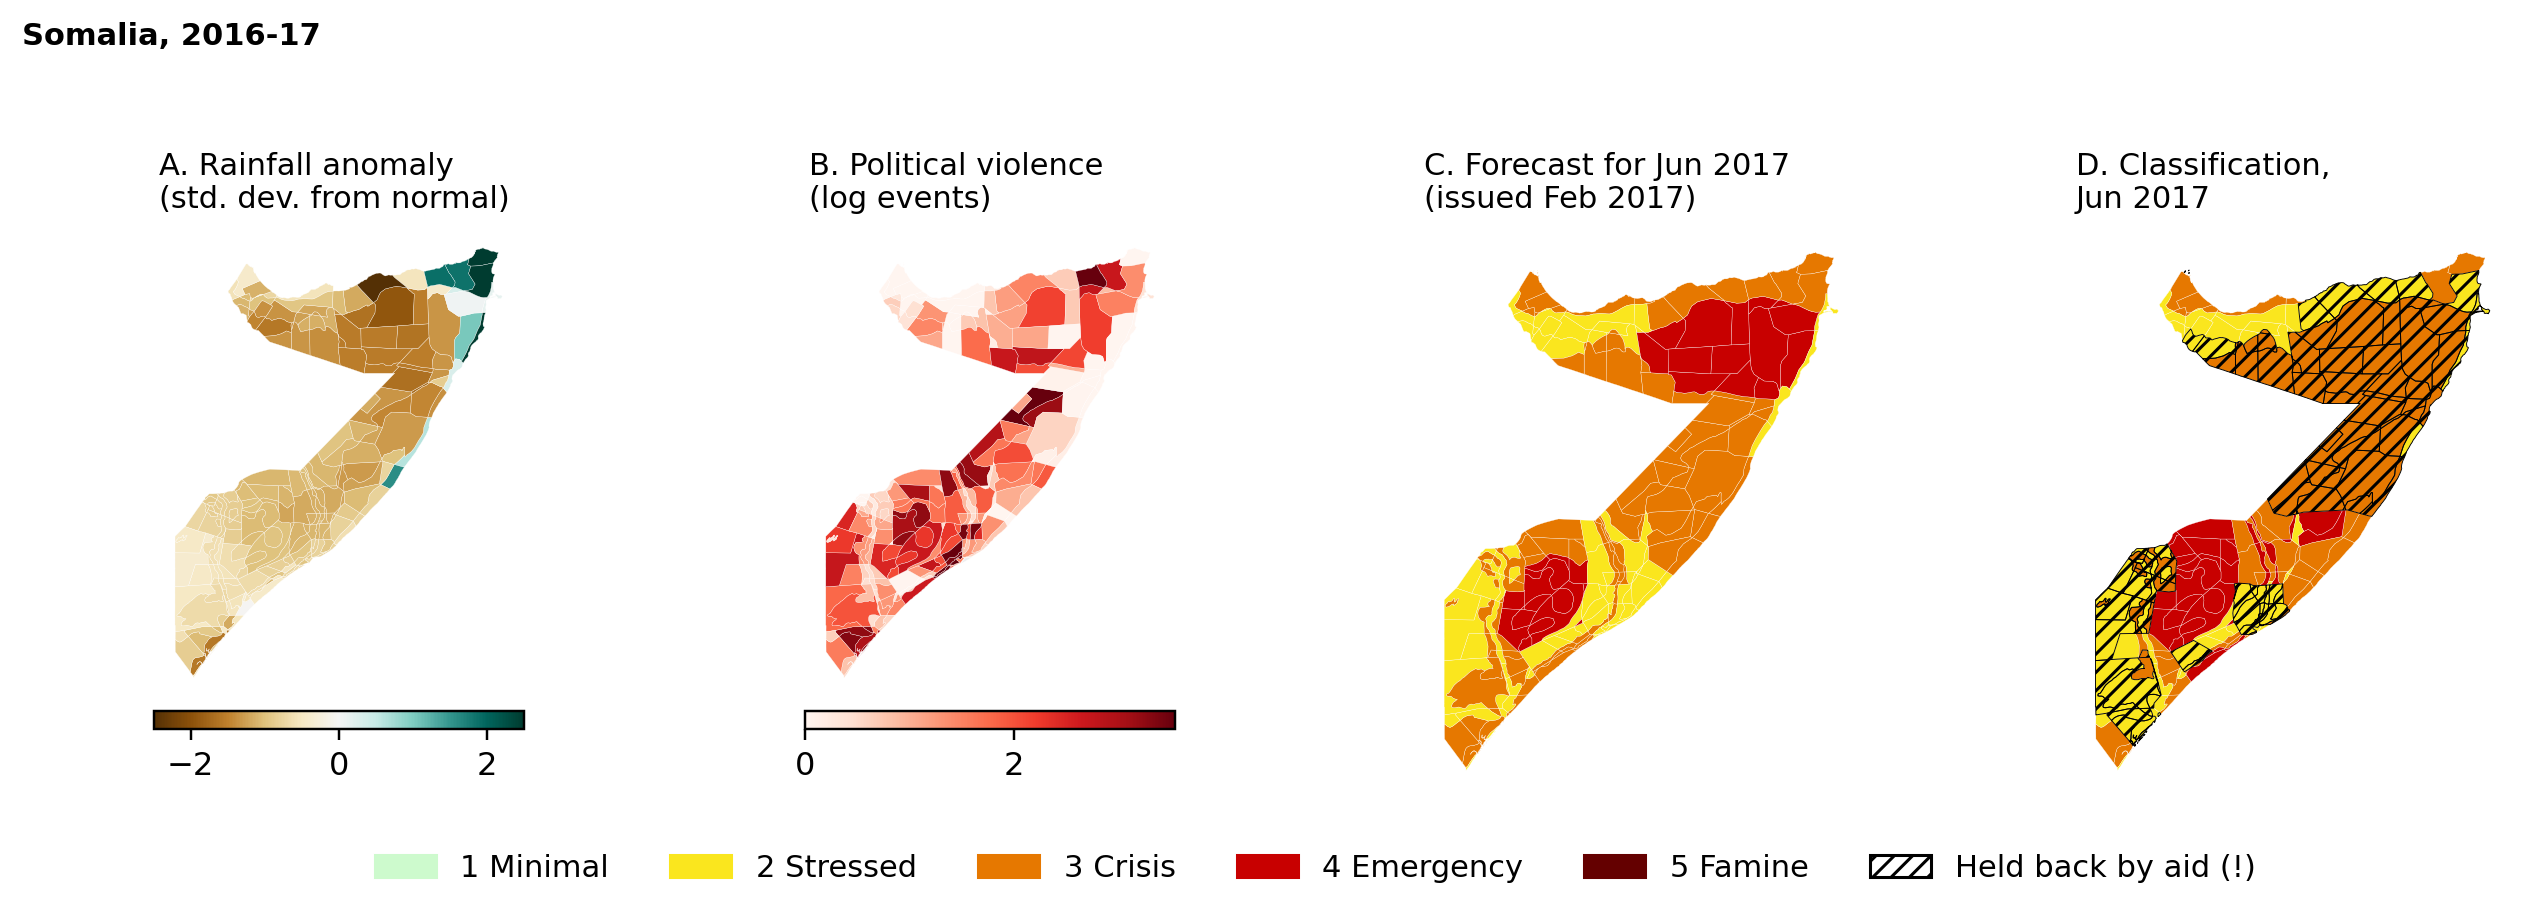
\includegraphics[width=\textwidth]{figures/fig_case_somalia.png}
\caption{Somalia, 2016--17. FEWS NET areas. A: rainfall over the six months to January 2017, in standard deviations from the same months in the previous 20 years (CHIRPS). B: political violence events in the six months to January 2017 (ACLED, log of one plus events). C: FEWS NET's forecast, issued February 2017, for June 2017. D: FEWS NET's classification for June 2017; hatching marks areas FEWS NET flagged as held at least one phase better by humanitarian assistance.}\label{fig:case_so}
\end{figure}

\begin{figure}[t]
\centering
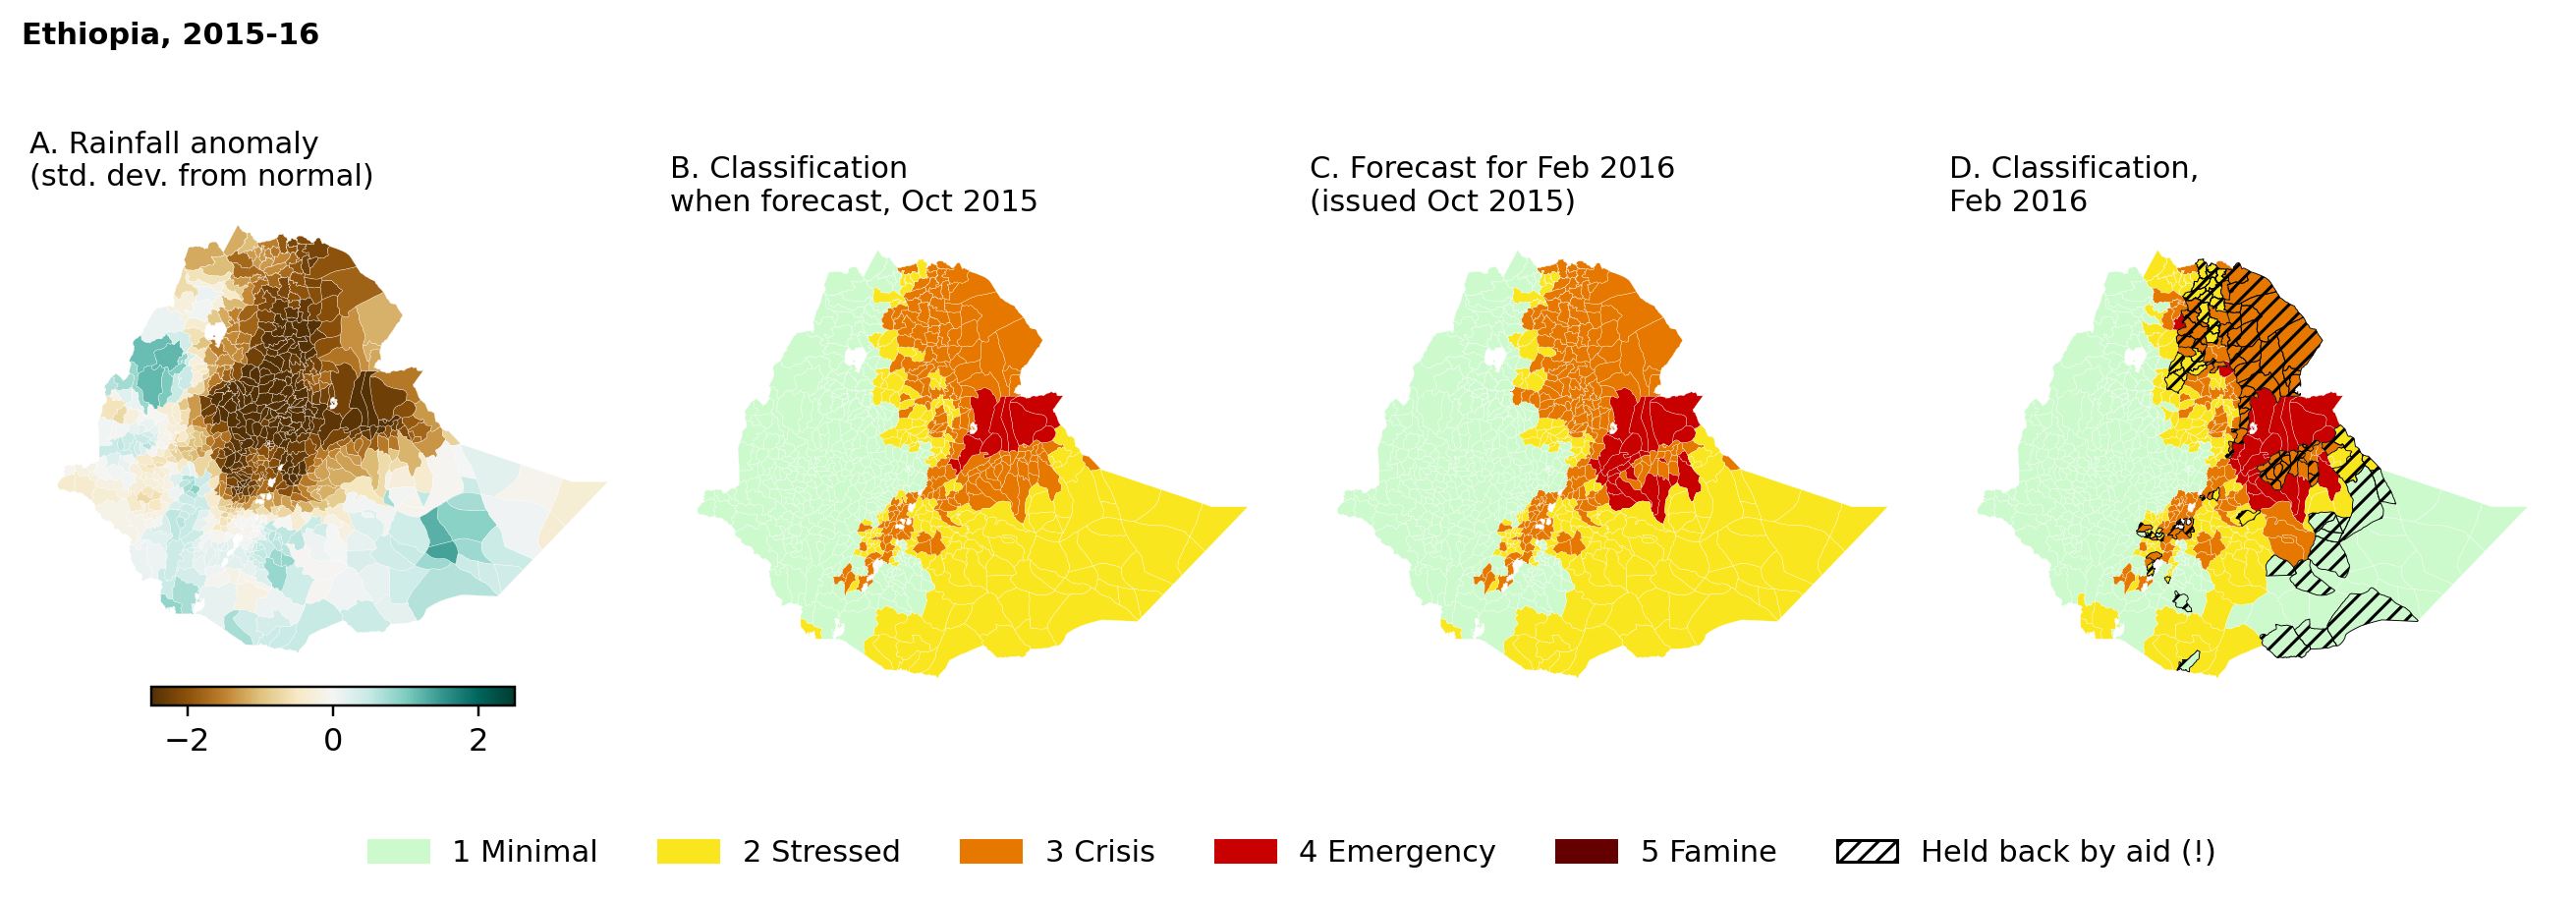
\includegraphics[width=\textwidth]{figures/fig_case_ethiopia.png}
\caption{Ethiopia, 2015--16. FEWS NET areas. A: rainfall over the six months to September 2015, in standard deviations from the same months in the previous 20 years (CHIRPS). B: FEWS NET's classification in October 2015, when the forecast was issued. C: FEWS NET's forecast, issued October 2015, for February 2016. D: FEWS NET's classification for February 2016; hatching marks areas FEWS NET flagged as held at least one phase better by humanitarian assistance.}\label{fig:case_et}
\end{figure}

\FloatBarrier
\section{Data}\label{sec:data}

Table~\ref{tab:data} summarizes the data. All sources are public; Appendix~\ref{app:data} gives details and match rates.

\begin{table}[t]
\centering
\begin{threeparttable}
\caption{Data sources}\label{tab:data}
\small
\begin{tabular}{L{4.3cm}L{6.0cm}L{4.4cm}}
\toprule
Source & Content & Coverage used \\
\midrule
FEWS NET Data Warehouse \citep{fewsnetdata} & Current-situation phases, near- and medium-term forecasts and aid flags for each FEWS NET area & \csAreaMonths{} area-months; \csAreas{} areas in \csCountries{} countries; 2011--2024 \\[3pt]
Cadre Harmonis\'e \citep{chdata} & Area classifications and projections, West and Central Africa & 2014--2026; district or region level \\[3pt]
IPC \citep{ipcdata} & Area classifications and projections outside West Africa & 2017--2026 \\[3pt]
Global Report on Food Crises \citep{GRFC2025} & People in Crisis or worse, by country and year & 2016--2024; \covCountries{} countries \\[3pt]
OCHA Financial Tracking Service \citep{OCHAFTS} & Humanitarian funding commitments by recipient, sector and date & 2011--2024 \\[3pt]
CHIRPS \citep{funk2015chirps} & Monthly rainfall, 0.05$^\circ$ grid (aggregated to 0.2$^\circ$) & 1981--2026 \\[3pt]
ACLED \citep{raleigh2010acled,acledhdx} & Political violence events and deaths by district and month & 19 countries with sub-national data \\[3pt]
WFP market prices \citep{wfpprices} & Retail prices of cereals and tubers by market & Nearest market within 150 km \\
\bottomrule
\end{tabular}
\begin{tablenotes}\footnotesize
\item \textit{Notes:} FEWS NET areas are livelihood zones or administrative units, depending on the country. IPC and Cadre Harmonis\'e areas are matched to FEWS NET areas by spatial overlay.
\end{tablenotes}
\end{threeparttable}
\end{table}

\paragraph{FEWS NET.} We use every current-situation map and forecast published through FEWS NET's data warehouse from January 2011 to December 2024 --- \csAreaMonths{} area-months in \csAreas{} areas and \csCountries{} countries. We stop at 2024 so that the 2025 shutdown does not distort the sample.

\paragraph{Independent classifications.} The Cadre Harmonis\'e covers 19 West and Central African countries from 2014 and the IPC some 30 countries from 2017. For each area and analysis, we record whether the area is classified in Crisis or worse and the share of its population in Crisis or worse, for both the current situation and the projection. We overlay these areas on FEWS NET's to compare like with like. These classifications are independent of FEWS NET's own maps, but not of its staff, who join many IPC and Cadre Harmonis\'e analyses. They are the best independent benchmark available, not a perfect one.

\paragraph{Funding.} The Financial Tracking Service records humanitarian commitments by recipient country and date. Over 2011--2024, FEWS NET countries received about \ftsShareFews{} percent of all humanitarian funding; the United States provided about \ftsUsFoodShare{} percent of food and nutrition funding to these countries. We sum commitments to each country over the six months after each FEWS NET map round.

\paragraph{Raw signals.} To represent what a donor could know without FEWS NET, we measure, for each FEWS NET area and round: rainfall over the previous 6 and 12 months relative to the same months in the preceding 20 years (CHIRPS); political violence events and deaths in the previous 6 months and their change on a year earlier (ACLED), apportioned from districts by area; and 3- and 12-month changes in retail cereal prices at the nearest WFP market. Rainfall covers 99 percent of area-rounds, conflict 48 percent and prices 28 percent; models treat missing values as missing.

\paragraph{Coverage.} Figure~\ref{fig:coverage} shows why FEWS NET matters. Over 2016--2024, the countries FEWS NET monitored accounted for \covPthree{} percent of the world's person-years in Crisis or worse, and \covPfour{} percent of those in Emergency or worse, across the \covCountries{} countries in the Global Report on Food Crises. The largest crises outside its coverage were Syria, Pakistan, Bangladesh and Myanmar.

\begin{figure}[t]
\centering
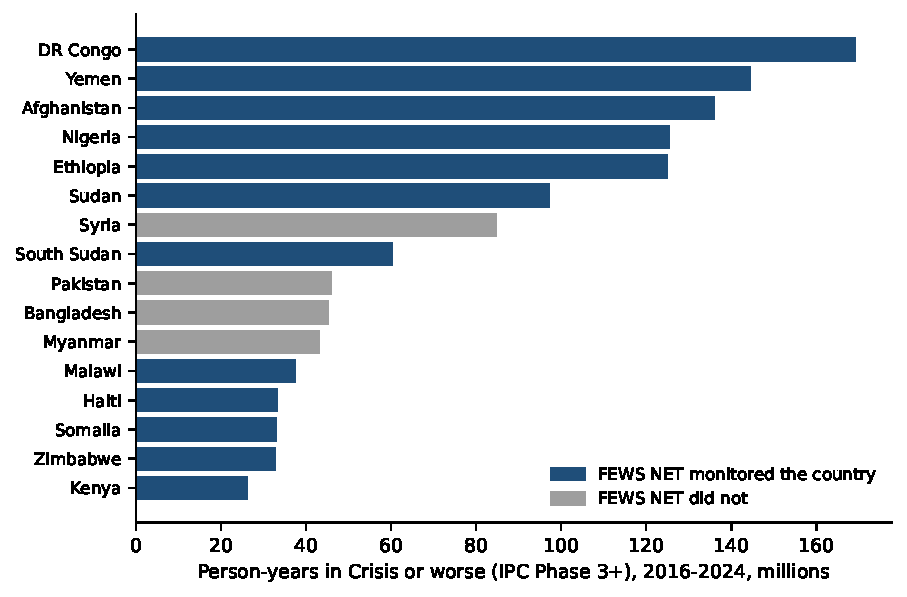
\includegraphics[width=0.85\textwidth]{figures/fig1_coverage.pdf}
\caption{Where the world's food crises are. Person-years in Crisis or worse (IPC Phase 3 and above), 2016--2024, for the 16 countries with the most, by whether FEWS NET monitored the country. Source: Global Report on Food Crises country-year database.}\label{fig:coverage}
\end{figure}

\section{Type II errors: missed emergencies}\label{sec:type2}

We define a new emergency as an area mapped in Emergency or worse whose previous map, no more than six months earlier, placed it below Emergency. Between 2011 and 2024 there were \tIIonsets{} such cases. For each, we look back at every forecast FEWS NET issued for that area and month in the preceding one to eight months.

Figure~\ref{fig:type2} shows the result. Panel A plots, by how far ahead the forecast was made, the share of new emergencies that FEWS NET forecast to be in Emergency (dark line) and in Crisis or worse (light line). Almost all new emergencies were foreseen as crises: at four months, \tIIleadfourCrisis{} percent had been forecast to be in at least Crisis. Few were foreseen as emergencies: \tIIleadeight{} percent at eight months, \tIIleadfour{} percent at four months and \tIIleadone{} percent one month ahead. Panel B gives the most severe forecast made four to eight months ahead --- the window that matters for mobilizing aid. \tIIearlyEmergency{} percent were forecast as Emergency, \tIIearlyCrisis{} percent as Crisis, and \tIIearlyStressed{} percent as Stressed or better.

\begin{figure}[t]
\centering
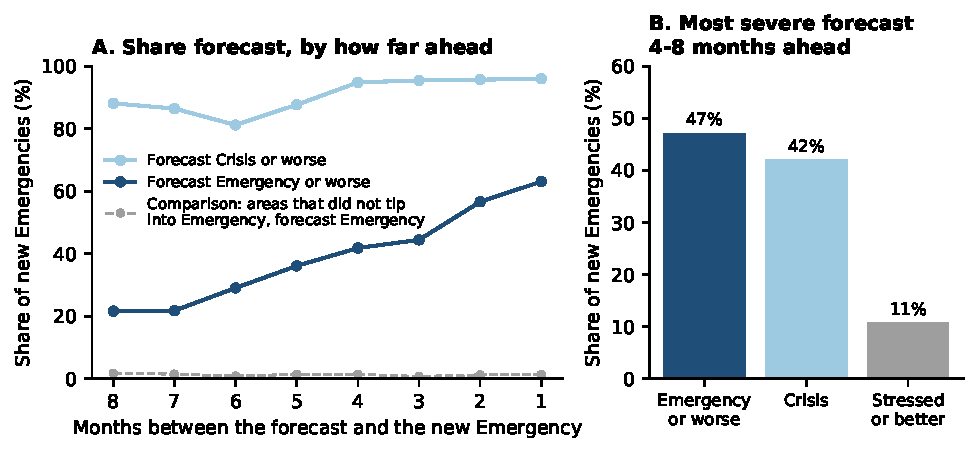
\includegraphics[width=\textwidth]{figures/fig2_type2.pdf}
\caption{Were new emergencies foreseen? \tIIonsets{} FEWS NET areas that entered Emergency or worse (IPC Phase 4+) in 2011--2024, after a previous map below Emergency. Panel A: share of these areas that FEWS NET had forecast, $k$ months earlier, to be in Emergency or worse (dark) or Crisis or worse (light), for the outcome month or the three months before it. The grey dashed line shows the share of areas that did \emph{not} tip into Emergency that were forecast to be in Emergency. Panel B: the most severe forecast issued four to eight months before the new emergency.}\label{fig:type2}
\end{figure}

These numbers say that FEWS NET's Type II errors are mostly errors of degree, not of kind. Only \tIInoWarning{} percent of new emergencies came with no warning of at least Crisis. The warnings also discriminate: four months ahead, FEWS NET forecast Emergency for \tIIleadfour{} percent of areas that went on to tip into Emergency, but for only \tIIcontrolEmergency{} percent (on average across horizons) of comparable areas that did not. What FEWS NET does badly is forecast escalation from Crisis to Emergency  --- the step at which, in the IPC's definitions, very high acute malnutrition and excess mortality are expected.

A wider lens tells the same story. Food security changes slowly: in \accNaive{} percent of area-rounds, an area's next map shows the same phase as its current one. FEWS NET's medium-term forecast matches the next map \accForecast{} percent of the time, against \accNaive{} percent for a forecast that nothing changes. Among the \shareChanges{} percent of area-rounds in which the phase did change, the forecast was right \accChanges{} percent of the time. These numbers score FEWS NET against itself and so flatter it, but the conclusion is consistent with earlier evaluations: most of FEWS NET's headline accuracy comes from stable areas, and its skill on change is real but partial.

\FloatBarrier
\section{Type I errors: false alarms}\label{sec:type1}

We define an emergency warning as a forecast, issued four to eight months ahead, that an area would be in Emergency or worse in a month for which FEWS NET later published a current-situation map. There were \tIwarnings{} such area-month warnings between 2011 and 2024.

Figure~\ref{fig:type1} shows what happened to them. In \tIcame{} percent of cases the area was in Emergency or worse, as forecast. In \tIfailed{} percent it was not. Almost all of those ended one phase lower, in Crisis; only \tIbetter{} percent ended in Stressed or better.

\begin{figure}[t]
\centering
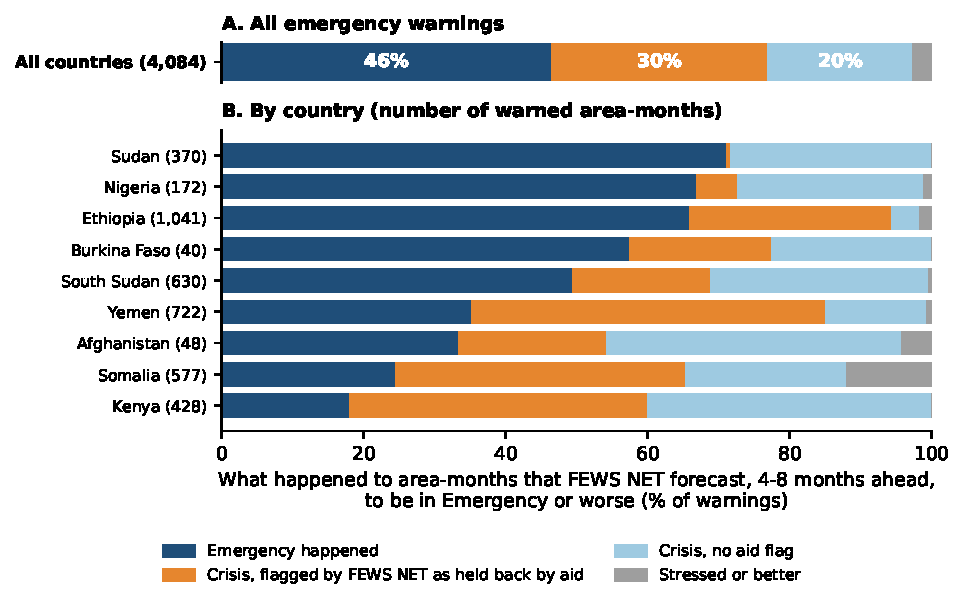
\includegraphics[width=0.95\textwidth]{figures/fig3_type1.pdf}
\caption{What happened to emergency warnings. Area-months that FEWS NET forecast, four to eight months ahead, to be in Emergency or worse (IPC Phase 4+), 2011--2024, by the phase FEWS NET later mapped. Panel A: all countries. Panel B: countries with at least 40 warned area-months. ``Held back by aid'' means FEWS NET's map carried its ``!'' flag: humanitarian assistance was keeping the area at least one phase better than it would otherwise be.}\label{fig:type1}
\end{figure}

FEWS NET's aid flag lets us ask how many of these apparent false alarms FEWS NET itself attributes to aid. Of the warned areas that ended in Crisis, \tIflagShareOfCrisis{} percent carried the flag, against \tIflagUnwarnedCrisis{} percent of Crisis areas that had not been warned about. Taken at face value, the flag reclassifies \tIflagged{} percent of all emergency warnings as crises held back by aid, leaving \tIunflagged{} percent ending in Crisis without the flag and \tIbetter{} percent ending lower. On this reading, about a quarter of FEWS NET's emergency warnings were genuine false alarms.

The pattern differs sharply across countries (Figure~\ref{fig:type1}, panel B). In Sudan, Nigeria and Ethiopia, two-thirds or more of emergency warnings came true. In Somalia and Kenya, fewer than a quarter did, and FEWS NET credited aid with holding back about half or more of the rest. In Sudan, where warnings failed, FEWS NET almost never credited aid.

Two checks suggest caution before crediting aid with the rest.

First, \tIflaggedAlreadyFlagged{} percent of the warned areas that ended in flagged Crisis had carried the flag on the map before the warning was issued. In those areas, the flag describes aid that was already flowing, not aid mobilized by the warning. The forecast should already have accounted for it, since FEWS NET's forecasts assume planned assistance. One reading is that FEWS NET forecast Emergency on the expectation that existing aid would fall away, and it did not; another is that the flag rationalizes a forecast that was too pessimistic. The data cannot distinguish them.

Second, if aid were preventing warned emergencies, warnings should come true less often when money then arrived. We test this in Appendix~\ref{app:masking} using FEWS NET's ``distinctive'' warnings --- the part of each forecast that rainfall, conflict, prices and the previous maps do not predict (Section~\ref{sec:value}). We compare countries whose humanitarian funding over the following six months rose more than their usual level and recent trend would predict with countries whose funding rose less. The share of distinctive warnings borne out is \maskMappedLow{} where funding rose less than usual and \maskMappedHigh{} where it rose more. Scoring against need (the mapped phase plus one if flagged) gives \maskNeedLow{} and \maskNeedHigh{}. We find no sign that funding surprises mask accuracy. Funding is only observed by country, so this test is coarse; it does not rule out well-targeted aid within countries.

Defining emergencies by need gives a similar picture. If we count an area as reaching Emergency when its mapped phase plus the aid flag reaches 4, there were \needOnsets{} such cases, and \needHeld{} percent were held back by aid on FEWS NET's own account. But \needHeldSteady{} percent of those held back were areas already in Crisis whose phase did not change; the flag simply switched on. And among these need-defined emergencies, early warning did not raise the share held back by aid (\needEarly{} percentage points, standard error \needEarlySe{}). FEWS NET's forecasts already assume the aid that is coming, so they are not designed to answer this question.

\FloatBarrier
\section{Does FEWS NET know something others don't?}\label{sec:value}

Accuracy against FEWS NET's own later maps says little about value. What matters for a funder is what would be lost without FEWS NET: its information relative to what donors could otherwise see, scored against outcomes it did not produce. We approach this in two ways.

\subsection{Against a world without FEWS NET}

We define two benchmarks for what donors would know without FEWS NET. The first uses only raw signals: local rainfall, conflict and food prices before the forecast, plus country and season. The second adds the latest official IPC or Cadre Harmonis\'e analysis of the area, if one was made in the previous eight months. The second benchmark is generous to the world without FEWS NET, because FEWS NET staff contribute to many official analyses. It is also usually unavailable: only \shareWithIndependent{} percent of FEWS NET's area-rounds had a recent official analysis.

For each benchmark, we use gradient-boosted trees to predict two things out of sample (each year predicted from models fitted on the other years): FEWS NET's own current map and forecast, and the outcome in the next official analysis. ``FEWS NET's contribution'' is the part of its map or forecast that the benchmark does not predict. We then score everything against the next independent IPC or Cadre Harmonis\'e analysis of the area. We focus on areas that were not in Crisis at the latest official analysis, because predicting that a crisis continues is easy. This leaves \aucN{} area-rounds in which \aucEvents{} areas tipped into Crisis.

Figure~\ref{fig:contribution} gives the main result as the area under the ROC curve (AUC): the probability that a randomly chosen area that tipped into Crisis is ranked above one that did not. Adding FEWS NET's map and forecast to the raw signals raises the AUC from \aucRaw{} to \aucRawFews{}, closing more than a quarter of the gap to perfect ranking. Adding them to the more generous benchmark raises it from \aucRawIPC{} to \aucRawIPCFews{}.

The second gain is small, and it is worth being clear about why it does not undercut the rest of the paper. First, it is measured where FEWS NET's alternatives are strongest. The benchmark includes the latest official analysis, which exists for only \shareWithIndependent{} percent of FEWS NET's area-rounds, and every observation in this test is, by construction, an area the IPC or Cadre Harmonis\'e covers. Second, those official analyses are not independent of FEWS NET: its analysts take part in them and its data feed them, so the benchmark already contains much of what FEWS NET knows. Third, the AUC is close to its ceiling; the move from \aucRawIPC{} to \aucRawIPCFews{} closes about an eighth of the remaining gap, and the regressions below find the gain precisely estimated. The fair reading is that where a recent official analysis exists, FEWS NET adds modestly to it. FEWS NET's distinctive value lies mainly where none exists --- three-quarters of its coverage --- and there we cannot score it against an independent outcome. Section~\ref{sec:money} shows that funding behaves accordingly.

\begin{figure}[t]
\centering
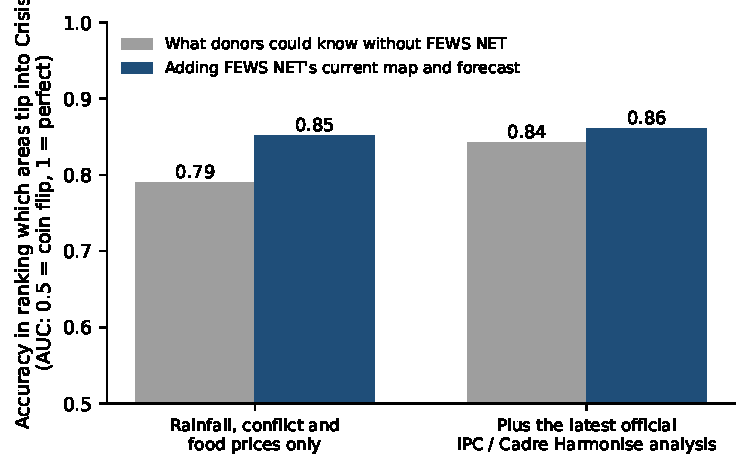
\includegraphics[width=0.7\textwidth]{figures/fig5_contribution.pdf}
\caption{FEWS NET's information beyond what donors could otherwise know. Accuracy in ranking which areas tip into Crisis or worse at the next official IPC or Cadre Harmonis\'e analysis, among \aucN{} area-rounds not in Crisis at the latest official analysis (\aucEvents{} tipped into Crisis), 2011--2024. Grey: out-of-sample predictions from rainfall, conflict, prices, country and season (left), plus the latest official analysis (right). Blue: the same models with FEWS NET's current map and forecast added. AUC is the probability that an area that tipped into Crisis is ranked above one that did not.}\label{fig:contribution}
\end{figure}

Table~\ref{tab:contribution} gives the regression version. The outcome is whether the area is in Crisis or worse at the next official analysis. We regress it on the benchmark's own prediction of that outcome and on FEWS NET's contribution, with country-by-round fixed effects, so the comparison is between areas in the same country at the same time:
\begin{equation*}
y_{a,t+1} = \alpha\, \hat{y}_{at} + \beta\, c_{at} + \mu_{c(a),t} + \varepsilon_{at},
\end{equation*}
where $y_{a,t+1}$ is an indicator for Crisis or worse in area $a$ at the next official analysis, $\hat{y}_{at}$ is the benchmark's prediction of it, $c_{at}$ is FEWS NET's contribution (its map or forecast minus the benchmark's prediction of that map or forecast), and $\mu_{c(a),t}$ is a country-by-round fixed effect. The coefficient $\beta$ measures how much of FEWS NET's distinctive signal is borne out by an independent assessment. Over the raw-data benchmark, it is \contribRawCur{} for the current map and \contribRawFc{} for the forecast when both enter (column 3); over the benchmark with official analyses, \contribRawIPCCur{} and \contribRawIPCFc{} (column 6). All are precisely estimated.

\begin{table}[t]
\centering

\caption{Is FEWS NET's distinctive information borne out by independent assessments?}\label{tab:contribution}
\scriptsize
\resizebox{\textwidth}{!}{\begin{tabular}{lcccccc}
\toprule
 & \multicolumn{3}{c}{Without FEWS NET: rainfall,} & \multicolumn{3}{c}{Without FEWS NET: rainfall, conflict,} \\
 & \multicolumn{3}{c}{conflict and prices} & \multicolumn{3}{c}{prices and latest official analysis} \\
\cmidrule(lr){2-4}\cmidrule(lr){5-7}
 & (1) & (2) & (3) & (4) & (5) & (6) \\
\midrule
FEWS NET current map, beyond the baseline & $0.201^{***}$ &  & $0.127^{***}$ & $0.165^{***}$ &  & $0.121^{***}$ \\
 & $(0.015)$ &  & $(0.023)$ & $(0.013)$ &  & $(0.020)$ \\
FEWS NET forecast, beyond the baseline &  & $0.195^{***}$ & $0.131^{***}$ &  & $0.142^{***}$ & $0.082^{***}$ \\
 &  & $(0.011)$ & $(0.019)$ &  & $(0.016)$ & $(0.023)$ \\
Baseline's own prediction (coefficient) & $0.42$ & $0.42$ & $0.44$ & $0.68$ & $0.68$ & $0.68$ \\
\midrule
Observations & 12,764 & 12,764 & 12,764 & 12,764 & 12,764 & 12,764 \\
Countries & 21 & 21 & 21 & 21 & 21 & 21 \\
AUC: baseline $\rightarrow$ adding FEWS NET & \multicolumn{3}{c}{0.79 $\rightarrow$ 0.85} & \multicolumn{3}{c}{0.84 $\rightarrow$ 0.86} \\
\bottomrule
\end{tabular}}
\par\vspace{4pt}\begin{minipage}{\textwidth}\scriptsize \textit{Notes:} Linear probability models. Outcome: area classified in Crisis or worse (IPC Phase 3+) at the next official IPC or Cadre Harmonis\'e analysis. Sample: official areas not in Crisis at the latest official analysis, 2011--2024. FEWS NET's map and forecast are overlaid onto official areas (share of the area in Crisis or worse). ``Beyond the baseline'' is FEWS NET's map or forecast minus its out-of-sample prediction from the baseline (gradient-boosted trees, fitted on other years). All columns control for the baseline's own out-of-sample prediction of the outcome and include country-by-round fixed effects. Standard errors clustered by country in parentheses. * $p<0.10$, ** $p<0.05$, *** $p<0.01$. The last row gives the AUC for ranking areas that tip into Crisis, using the baseline alone and adding FEWS NET's map and forecast.
\end{minipage}

\end{table}

The coefficients are well below one. Only part of FEWS NET's distinctive signal shows up in the next official assessment. Some of the gap is noise in FEWS NET's judgments, some is noise in the official assessments, and some, if aid works, is masking. But the signal is clearly there, and it survives controlling for the official analyses that do exist.

\subsection{Head to head with the official projections}

The IPC and Cadre Harmonis\'e also publish forecasts. Where both exist, we compare FEWS NET's forecast with the official projection for the same area and period, both scored against the next official current analysis. We match each official projection to FEWS NET's forecast from its latest round at or up to four months before the official analysis. This gives \offNall{} area-projections in \offCountriesAll{} countries; \offN{} of them were not in Crisis at the latest official analysis, and \offNew{} of those tipped into Crisis. In the Cadre Harmonis\'e, projections target the June--August lean season, which is rarely assessed as a current period; we score them against the next current analysis (September--December). Both forecasters face the same mismatch.

Figure~\ref{fig:official} plots both forecasts in Type I/Type II space. The vertical axis is the share of new crises that were not warned about (misses); the horizontal axis is the share of areas that stayed out of Crisis but were warned about (false alarms). The official projection classifies the area in Crisis for \offHitOfficial{} percent of new crises, at a false alarm rate of \offFaOfficial{} percent. FEWS NET forecasts Crisis for most of the area in \offHitFews{} percent of new crises, at a false alarm rate of \offFaFews{} percent. FEWS NET is more conservative: it misses slightly more but cries wolf less. The two are complements. Warning when either one warns catches \offHitEither{} percent of new crises at a false alarm rate of \offFaEither{} percent. In \offHitOnlyFews{} percent of new crises, FEWS NET warned and the official projection did not.

\begin{figure}[t]
\centering
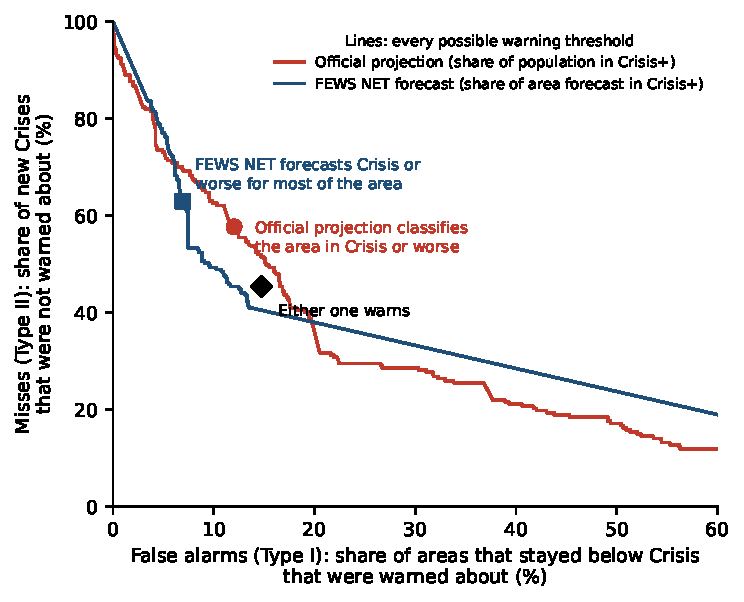
\includegraphics[width=0.72\textwidth]{figures/fig4_official.pdf}
\caption{FEWS NET and the official projections in Type I/Type II space. \offN{} official IPC and Cadre Harmonis\'e areas not in Crisis at the latest official analysis, in \offCountries{} countries, \offYears{}; \offNew{} tipped into Crisis at the next official analysis. Points: misses (new crises not warned about) and false alarms (areas warned about that stayed out of Crisis) for the official projection classifying the area in Crisis or worse, FEWS NET forecasting Crisis or worse for most of the area, and either one warning. Lines trace every warning threshold for the official projection (share of the population projected in Crisis or worse) and for FEWS NET (share of the area forecast in Crisis or worse). Lower and further left is better.}\label{fig:official}
\end{figure}

Table~\ref{tab:official} regresses the next official classification on both forecasts. FEWS NET's forecast predicts the outcome over and above the official projection. With both forecasts and the latest official analysis (column 4), the coefficient on FEWS NET's forecast is \offCoefAllFews{} and on the official projection \offCoefAllProj{}. For areas not yet in Crisis (Panel B, column 3), they are \offCoefNewFews{} and \offCoefNewProj{}. With only 12 to 14 countries, cluster-robust standard errors can overstate precision; wild cluster bootstrap $p$-values for FEWS NET's coefficient are \bootOffAllFews{} and \bootOffNewFews{}.

\begin{table}[t]
\centering

\caption{FEWS NET's forecasts and the official projections, scored against the next official analysis}\label{tab:official}
\scriptsize
\resizebox{\textwidth}{!}{\begin{tabular}{lccccc}
\toprule
 & (1) & (2) & (3) & (4) & (5) \\
\midrule
\multicolumn{6}{l}{\textit{A. All areas}} \\
Official projection: Crisis or worse & $0.220^{***}$ &  & $0.137^{***}$ & $0.056^{***}$ & $0.054^{***}$ \\
 & $(0.057)$ &  & $(0.030)$ & $(0.018)$ & $(0.017)$ \\
FEWS NET forecast: share of area in Crisis or worse &  & $0.329^{***}$ & $0.239^{***}$ & $0.178^{***}$ & $0.106^{***}$ \\
 &  & $(0.063)$ & $(0.048)$ & $(0.046)$ & $(0.037)$ \\
Latest official analysis: Crisis or worse &  &  &  & $0.275^{***}$ & $0.261^{***}$ \\
 &  &  &  & $(0.027)$ & $(0.024)$ \\
FEWS NET current map: share of area in Crisis or worse &  &  &  &  & $0.127^{**}$ \\
 &  &  &  &  & $(0.056)$ \\
Observations & 6,683 & 6,683 & 6,683 & 6,559 & 6,559 \\
Countries & 14 & 14 & 14 & 14 & 14 \\
\midrule
\multicolumn{6}{l}{\textit{B. Areas not in Crisis at the latest official analysis}} \\
Official projection: Crisis or worse & $0.104^{***}$ &  & $0.054^{***}$ & $0.054^{***}$ & $0.056^{***}$ \\
 & $(0.015)$ &  & $(0.014)$ & $(0.014)$ & $(0.014)$ \\
FEWS NET forecast: share of area in Crisis or worse &  & $0.179^{***}$ & $0.149^{***}$ & $0.149^{***}$ & $0.104^{**}$ \\
 &  & $(0.035)$ & $(0.033)$ & $(0.033)$ & $(0.041)$ \\
FEWS NET current map: share of area in Crisis or worse &  &  &  &  & $0.094$ \\
 &  &  &  &  & $(0.110)$ \\
Observations & 4,128 & 4,128 & 4,128 & 4,128 & 4,128 \\
Countries & 12 & 12 & 12 & 12 & 12 \\
\bottomrule
\end{tabular}}
\par\vspace{4pt}\begin{minipage}{\textwidth}\scriptsize \textit{Notes:} Linear probability models. Outcome: area classified in Crisis or worse (IPC Phase 3+) at the next official IPC or Cadre Harmonis\'e current analysis after the projection. Official projection: Cadre Harmonis\'e March projections for June--August, and IPC first projections. FEWS NET forecast: share of the official area that FEWS NET's latest forecast (issued up to four months before the official analysis) placed in Crisis or worse for the projection period. All columns include country-by-analysis-round fixed effects. In Panel B, the latest official analysis is constant by construction, so column (4) repeats column (3). Standard errors clustered by country in parentheses; with 12--14 clusters, see wild bootstrap $p$-values in the text. * $p<0.10$, ** $p<0.05$, *** $p<0.01$.
\end{minipage}

\end{table}

These comparisons are partly circular: FEWS NET analysts join many official analyses, and both teams read each other's work. That makes it more notable, not less, that FEWS NET's forecast keeps predictive power after controlling for the official projection.

\FloatBarrier
\section{Does money follow the warnings?}\label{sec:money}

Information has value only if someone acts on it. We cannot observe aid at the level of FEWS NET's areas, so we ask whether humanitarian funding to a country moves with FEWS NET's classifications of that country. For each country and FEWS NET round, we regress the log of humanitarian funding committed over the next six months on the share of the country's FEWS NET areas in Crisis or worse on the current map, and on the share forecast to be in Crisis or worse four to eight months ahead.

Across countries, funding follows FEWS NET's maps closely. Without controls, and holding the current map fixed, a 10 percentage point rise in the share of a country's areas forecast to be in Emergency goes with \aidAllFourFcPool{} percent more humanitarian funding (95 percent interval \aidAllFourFcPoolCi{}). Most of this reflects persistent differences between countries: large, chronic crises get both bad maps and more money. Figure~\ref{fig:money}A shows what survives as controls are added for global funding swings, the country's funding in the previous six months, and the country's usual aid level. With all controls, the current map no longer predicts funding (\aidFoodThreeCurWithin{} percent for food and nutrition funding per 10 percentage points of areas in Crisis), but the forecast does (\aidFoodThreeFcWithin{} percent; interval \aidFoodThreeFcWithinCi{}). Within a country, money moves when FEWS NET expects things to get worse, not when it reports that they are bad. The Emergency shares are too rarely nonzero within countries to estimate this precisely (Appendix Table~\ref{tab:money}).

\begin{figure}[H]
\centering
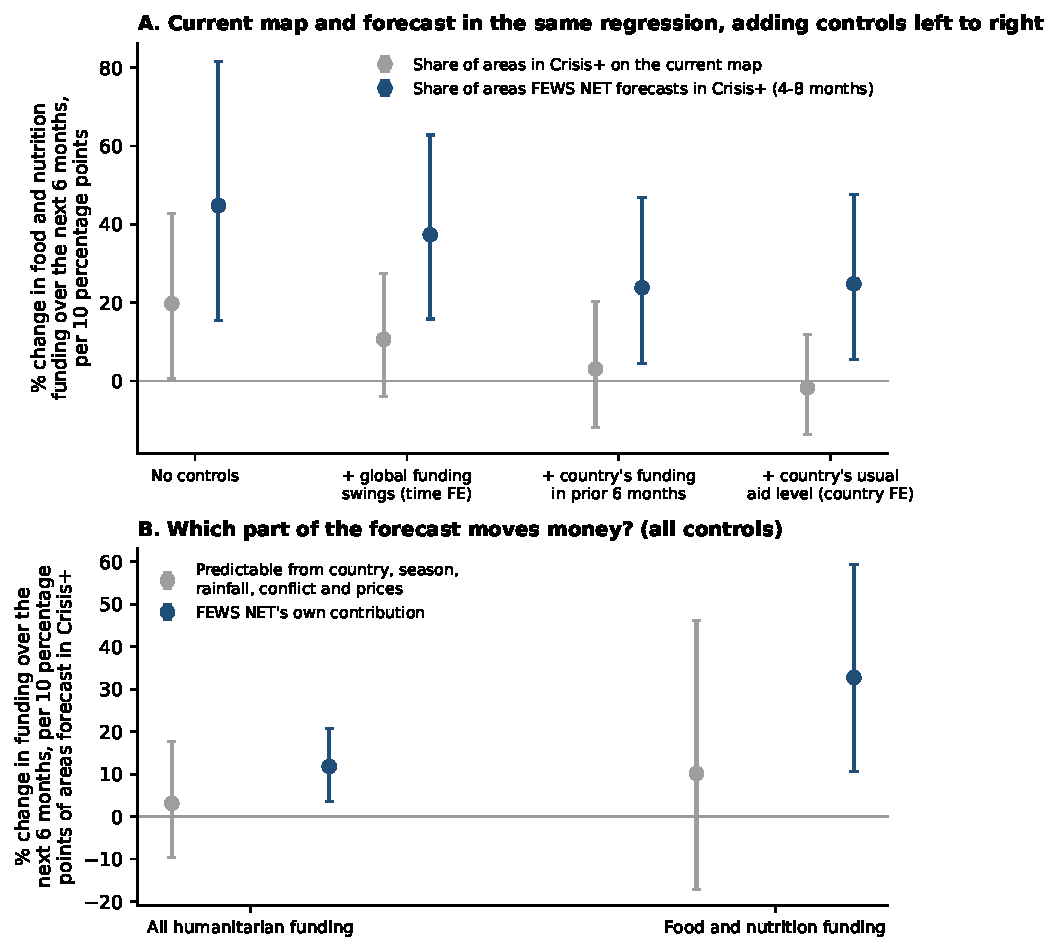
\includegraphics[width=0.92\textwidth]{figures/fig6_money.pdf}
\caption{Does humanitarian funding follow FEWS NET? Country $\times$ FEWS NET round, 2011--2024. Outcome: humanitarian funding committed to the country over the next six months (OCHA Financial Tracking Service, log), expressed as the percent change per 10 percentage points more of the country's FEWS NET areas in Crisis or worse. Panel A: the share in Crisis or worse on the current map and the share forecast in Crisis or worse four to eight months ahead, in the same regression, adding controls from left to right. Panel B: the forecast split into the part predictable from rainfall, conflict, prices, country and season, and FEWS NET's own contribution; with time and country fixed effects and funding in the previous six months. 95 percent intervals clustered by country.}\label{fig:money}
\end{figure}

Does funding respond to FEWS NET's own information, or to the rainfall failures and conflict that donors could see directly? Panel B splits the forecast into the part predictable from the country, the season and raw signals, and FEWS NET's contribution. The predictable part is mostly country and season: those alone account for \predCountrySeason{} percent of its variation, and within a country and season, rainfall, conflict and prices explain only \predShocksWithin{} percent of the variation in FEWS NET's forecasts. Across country-rounds, the predictable part varies little within countries (standard deviation \predBaseSdWithin{}, against \predBaseSd{} overall), while FEWS NET's contribution varies almost entirely within them (\predContribSdWithin{} of \predContribSd{}). Only the contribution predicts funding: \moneyRawAllContrib{} percent more humanitarian funding (interval \moneyRawAllContribCi{}) and \moneyRawFoodContrib{} percent more food and nutrition funding (\moneyRawFoodContribCi{}) per 10 percentage points of areas FEWS NET forecasts in Crisis beyond what that information predicts. The predictable part has no detectable effect (\moneyRawAllBase{} and \moneyRawFoodBase{} percent, with wide intervals). Results are similar against the benchmark that includes official analyses (Table~\ref{tab:money}). Funding follows FEWS NET's distinctive information more strongly where official analyses are scarce. In country-rounds where fewer than half of FEWS NET's areas had a recent official analysis (\hetShareHigh{} percent of country-rounds have more), a 10 percentage point rise in its distinctive forecast comes with \hetAllLow{} percent more humanitarian funding and \hetFoodLow{} percent more food funding. Where official analyses are common, the figures are \hetAllHigh{} and \hetFoodHigh{} percent. The difference is imprecise (standard errors \hetAllDiffSe{} and \hetFoodDiffSe{} log points per unit), but it matches the pattern in Section~\ref{sec:value}.

These are associations, not causal effects. Donors and FEWS NET may respond to the same news that our raw signals miss --- a displacement wave, a government request, a news story. But the pattern is the one we would expect if FEWS NET's forecasts inform allocation: funding responds to the forward-looking, distinctive part of FEWS NET's analysis, and not to what anyone could infer from a country's usual situation and public data.

\FloatBarrier
\section{What does a phase mean for lives?}\label{sec:phase}

Everything so far concerns FEWS NET's phases: whether it forecasts them well, and whether money follows them. To turn phases into lives, the next section needs to know how many more children are malnourished, and how many more people die, in an area that is one phase worse. The usual answer is the IPC's reference table, which ties each phase to a band of crude death rates (below 0.5 deaths per 10,000 people per day in Phases 1 and 2, 0.5--1 in Crisis, 1--2 in Emergency and above 2 in Famine) and of acute malnutrition among children under five (below 5, 5--10, 10--15, 15--30 and above 30 percent) \citep{IPC2021manual,ipcreftable}. This section asks whether measured outcomes follow those bands. We know of no study that systematically compares survey-measured child wasting or mortality with the acute food insecurity phase of the same area across countries, or that scores IPC, Cadre Harmonis\'e or FEWS NET classifications against anthropometry or mortality measured later. The closest evidence is fragmentary. The IPC's own guidance notes that acute food insecurity and acute malnutrition phases often diverge --- in 2020 only 3 of 9 districts of Karamoja in Uganda had the same phase on both scales --- but reports no systematic statistics \citep{ipc2024linkages}. A Somalia forecasting study includes the district share of the population in Phase 3 or worse among many candidate predictors of acute malnutrition, and finds it significant, without reporting its size \citep{reusken2025}. Mortality studies use IPC phases only to define baseline periods or as a visual cross-check \citep{checchi2013,warsame2023,ratnayake2025smed}, and a recent review concludes that the link between food insecurity and mortality in humanitarian settings cannot be answered with current evidence \citep{annan2023elrha}.

\subsection{Why the bands may not hold}

The bands were not derived from food insecurity data. They descend from 1980s and 1990s benchmarks for refugee camps: a doubling of a baseline crude death rate of about 0.44, and camp-based relations between wasting and mortality \citep{youngjaspars2009}. When the IPC created a separate scale for acute malnutrition in 2016, it noted that food insecurity and acute malnutrition do not always match, in either direction \citep{ipc2016amn}. Acute malnutrition depends on disease, water, sanitation and care as well as food. A meta-analysis of household studies finds that food insecurity predicts stunting and underweight but not wasting \citep{moradi2019}, and studies in Chad, Darfur, South Sudan and Niger find wasting hotspots that do not coincide with food-insecurity hotspots \citep{youngmarshak2017,luc2023chad}. In Somalia, models that forecast acute malnutrition lean mainly on its own past values \citep{checchi2022malnut,reusken2025}, and a FEWS NET causal analysis in Niger found household food insecurity not independently associated with wasting \citep{mcdonald2017nca}.

\subsection{Method}

We use three kinds of evidence. First, survey measurements matched to FEWS NET's phase for the same area and time. For a survey of area $a$ in season $t$, with measured outcome $y_{at}$ (acute malnutrition, or a crude or under-five death rate) and FEWS NET phase $P_{at}$ (its forecast for the survey month, or its map), we estimate
\begin{equation*}
y_{at} = \beta P_{at} + \mu_a + \lambda_t + \varepsilon_{at}.
\end{equation*}
Without the area effects $\mu_a$, $\beta$ compares different areas: are areas in worse phases worse off? With them, it compares the same area over time: when an area is one phase worse than usual, how much worse are its outcomes? The second is what the benefit-cost calculation needs, since it asks what happens when aid holds a given area one phase better. The season effects $\lambda_t$ remove shocks common to the country in a season. We also score FEWS NET's forecast as a predictor of $y_{at}$ out of sample, leaving out one season at a time, against the simplest alternative: the area's own measurement in the previous round.

Which surveys are used matters. Surveys sent where trouble is suspected will overstate the link between phase and outcome, because they are fielded where both are bad (Section~\ref{sec:pieces}). So we rely mainly on scheduled surveys, fielded on a fixed calendar whatever the conditions, and treat ad hoc surveys as an upper bound. Second, we compare the IPC's two scales, for acute food insecurity and for acute malnutrition, where both classify the same area. Third, we compare the excess deaths estimated in documented crises with the number of people in Crisis or worse.

\subsection{Somalia's scheduled surveys}

Somalia's Food Security and Nutrition Analysis Unit (FSNAU), managed by FAO, surveys the country's rural livelihood zones, towns and displaced settlements twice a year, after the Gu and Deyr rains, on a fixed calendar. We assembled all \fsAll{} survey results it published from late 2010 to 2026, from its results portal and its technical reports. We kept the rural SMART surveys run by FSNAU itself and matched each surveyed zone to FEWS NET's mapping units by livelihood zone and region. That leaves \fsN{} zone-seasons in \fsZones{} zones over \fsSeasons{} seasons with FEWS NET's forecast, its current map and the zone's result from the previous round. Mean acute malnutrition was \fsGam{} percent, and \fsCrit{} percent of zone-seasons were at or above the critical level of 15 percent. Two caveats apply. Insecure zones of south-central Somalia, notably Juba, South Gedo and parts of Bakool and Hiran, were often skipped or assessed only by arm-circumference screening, so the worst-hit areas are under-represented. And FSNAU's analysts work alongside FEWS NET's, though the survey measurements are independent of the classifications.

Across zones, FEWS NET's phases do not track measured malnutrition (Figure~\ref{fig:fsnau}). Mean acute malnutrition was \fsGamTwo{} percent in zones FEWS NET forecast to be Stressed or better, \fsGamThree{} percent in zones forecast to be in Crisis and \fsGamFour{} percent in zones forecast to be in Emergency or worse. The correlation between FEWS NET's forecast, issued a median of \fsLead{} months ahead, and the measured rate is \fsCorrFc{}. The correlation with FEWS NET's map published just after the survey, which could draw on its results, is \fsCorrAfter{}. The zone's own result six months earlier correlates \fsCorrLag{} with this round's. Out of sample, the previous survey explains \fsRtwoLag{} of the variance in acute malnutrition, and FEWS NET's forecast explains none ($R^2$ of \fsRtwoFc{}); adding the forecast to the previous survey does not help (\fsRtwoBoth{}). For predicting whether a zone reaches the critical level, the AUC is \fsAucLag{} with the previous survey and \fsAucFc{} with FEWS NET's forecast. The same holds for under-five death rates: out-of-sample $R^2$ of \fsMortLag{} for the previous survey and \fsMortFc{} for the forecast.

Within zones there is a gradient, but a small one. When FEWS NET forecast a zone to be one phase worse than usual, its acute malnutrition was \wzGamZone{} points higher (standard error \wzGamZoneSe{}), or \wzGamZoneSeason{} points (\wzGamZoneSeasonSe{}) with season effects. Its crude death rate was \wzCdrZone{} deaths per 10,000 per day higher (\wzCdrZoneSe{}), or \wzCdrZoneSeason{} (\wzCdrZoneSeasonSe{}) with season effects, and its under-five death rate \wzUfiveZone{} (\wzUfiveZoneSe{}) or \wzUfiveZoneSeason{} (\wzUfiveZoneSeasonSe{}) higher. Using FEWS NET's map after the survey instead of its forecast gives similar estimates. At their midpoints, the IPC bands imply 5 points of acute malnutrition and 0.45 deaths per 10,000 per day for a step from Stressed to Crisis, and 10 points and 0.75 deaths for a step from Crisis to Emergency. The estimates may be biased down: the phase of a survey zone averages several FEWS NET units, which adds noise, and the worst-hit zones are under-surveyed. They are consistent with \citet{reusken2025}, who find that the official share of a district's population in Phase 3 or worse helps predict its acute malnutrition: a link exists, but it is far weaker than the bands imply.

\begin{figure}[t]
\centering
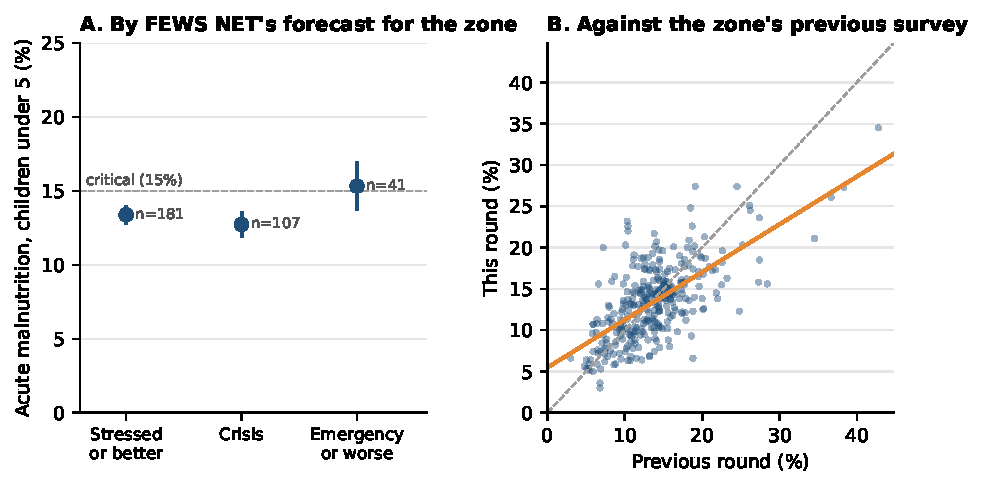
\includegraphics[width=0.92\textwidth]{figures/fig9_fsnau.pdf}
\caption{Scheduled surveys in Somalia: measured acute malnutrition against FEWS NET's forecast and the zone's previous survey. \fsN{} rural zone-seasons surveyed by FSNAU (SMART, weight-for-height), 2011--2024. Panel A: mean global acute malnutrition among children under five by FEWS NET's forecast phase for the zone, issued 3--8 months before the survey (mean over the FEWS NET units in the zone, rounded); 95 percent intervals. Panel B: this round's rate against the same zone's rate in the previous round, six months earlier; the orange line is the least-squares fit and the dashed line marks equality.}\label{fig:fsnau}
\end{figure}

\subsection{Other countries}

We repeated the comparison with two open sources. The SMART+ dashboard run by Action Against Hunger and UNICEF holds \spN{} survey results from 2022 to 2026, mostly from Nigeria, Ethiopia and Mozambique, \spNfews{} of which fall in FEWS NET's maps; \spNround{} come from Nigeria's recurring UNICEF survey rounds and the rest are ad hoc. FEWS NET's data warehouse holds \fdwN{} results from national survey rounds in Burkina Faso and Mauritania, 2003--2018.\footnote{The warehouse lists several thousand Ethiopian survey results as public, but does not return their values.} The gradient is steeper than in Somalia but still well below the bands. In SMART+, mean acute malnutrition was \spGamOne{}, \spGamTwo{}, \spGamThree{} and \spGamFour{} percent in areas FEWS NET mapped in Phases 1, 2, 3 and 4 or worse (correlation \spCorr{}); the jump at Phase 4 comes mostly from a dozen ad hoc surveys in Ethiopia. With country-by-year effects, one phase goes with \spSlope{} points of acute malnutrition (standard error \spSlopeSe{}). Nigeria's recurring rounds give \ngSlope{} points (\ngSlopeSe{}) per Cadre Harmonis\'e phase, and the Burkina Faso and Mauritania rounds \fdwSlope{} (\fdwSlopeSe{}) per FEWS NET phase. Crude death rates do not rise with FEWS NET's phase at all: \spCdrOne{}, \spCdrTwo{}, \spCdrThree{} and \spCdrFour{} deaths per 10,000 per day across the four groups (slope \spCdrSlope{}, standard error \spCdrSlopeSe{}). Against the official IPC or Cadre Harmonis\'e phase, they rise by \spCdrSlopeIpc{} per phase (\spCdrSlopeIpcSe{}).

The IPC's own two scales tell the same story. Where an area has both an acute food insecurity phase and an acute malnutrition phase for the same period, the two correlate \amnExpCorr{} and agree exactly in \amnExpAgree{} percent of \amnExpN{} areas in the Democratic Republic of Congo, Nigeria and South Sudan. Classifying acute malnutrition from published prevalence in \amnDerCountries{} countries gives a correlation of \amnDerCorr{} across \amnDerN{} areas.

\subsection{Excess deaths in documented crises}

The most direct evidence on mortality comes from crises whose death tolls have been estimated. Dividing estimated excess deaths by the number of people in Crisis or worse gives an excess death rate per person in Phase 3 or worse of roughly 0.15--0.2 per 10,000 per day in Somalia's 2017--18 and 2022 droughts \citep{warsame2023,lshtm2023somalia,ouchtar2026}, about 0.9 in northeast Nigeria in 2016--19 \citep{checchi2023nigeria}, and 1.1--1.9 in the 2010--12 Somalia famine, which met a late response \citep{checchi2013}. Measured crude death rates in areas reviewed for famine since 2017 have mostly been between 0.3 and 1.9, below the IPC's famine threshold of 2 \citep{ipcfrc2022somaliadec,ipcfrc2024sudandec}. Arithmetic with the IPC bands would have predicted roughly two to five times the excess deaths estimated for Somalia in 2022.

\subsection{A calibration}

Table~\ref{tab:calibration} summarizes the evidence and the values we use in Section~\ref{sec:bcr}. For each step from one phase to the next below Famine, we use \calCdrMid{} extra deaths per 10,000 per day (range \calCdrLo{}--\calCdrHi{}) and \calGamMid{} points of acute malnutrition (range \calGamLo{}--\calGamHi{}). For the step from Emergency to Famine, where the evidence comes from famines with a late response, we use \calFamMid{} extra deaths (range \calFamLo{}--\calFamHi{}). The central values are a fifth to a half of what the IPC bands imply for ordinary steps, and the low end of the range comes from Somalia's scheduled surveys, the most selection-free evidence we have.

\begin{table}[t]
\centering
\caption{What one phase means: evidence and the values used in the benefit-cost calculation}\label{tab:calibration}
\scriptsize
\begin{tabular}{L{5.6cm}L{2.6cm}L{3.0cm}}
\toprule
Evidence & Acute malnutrition (points per phase) & Crude death rate (per 10,000 per day, per phase) \\
\midrule
IPC reference bands, midpoints (Stressed to Crisis; Crisis to Emergency) & 5; 10 & 0.45; 0.75 \\
Somalia, scheduled surveys, within zones & \wzGamZoneSeason{}--\wzGamZone{} & \wzCdrZoneSeason{}--\wzCdrZone{} \\
SMART+ surveys, country-by-year effects & \spSlope{} & \spCdrSlope{} (FEWS NET); \spCdrSlopeIpc{} (IPC/CH) \\
Nigeria recurring rounds; Burkina Faso and Mauritania rounds & \ngSlope{}; \fdwSlope{} & -- \\
Excess deaths per person in Crisis or worse: Somalia 2017--18, 2022 & -- & 0.15--0.2 \\
Excess deaths per person in Crisis or worse: famines with late response & -- & 0.9--1.9 \\
\midrule
\textbf{Used below Famine} (central; range) & \calGamMid{}; \calGamLo{}--\calGamHi{} & \calCdrMid{}; \calCdrLo{}--\calCdrHi{} \\
\textbf{Used from Emergency to Famine} & -- & \calFamMid{}; \calFamLo{}--\calFamHi{} \\
\bottomrule
\end{tabular}
\par\vspace{4pt}\begin{minipage}{\textwidth}\scriptsize \textit{Notes:} Survey estimates are slopes of the measured outcome on the phase; Somalia within-zone estimates with zone effects, with and without season effects. IPC reference bands: differences between band midpoints. Excess deaths per person in Crisis or worse are estimated excess deaths divided by the person-days in IPC Phase 3 or worse; see text for sources.\end{minipage}
\end{table}

\FloatBarrier
\section{What is FEWS NET worth? A rough benefit-cost calculation}\label{sec:bcr}

The evidence so far is about information and money, not lives. This section pushes it as far as it will go toward a cost per death averted, using five pieces. Each is uncertain, and we show how the answer moves with each. The calculation is a guide to orders of magnitude, not an estimate of causal effects.

\paragraph{1. Cost.} Federal contract records show FEWS NET's cost directly \citep{usaspending}. Obligations under FEWS NET's contracts averaged \$\obAvgLong{} million a year over fiscal years 2017--2024 and \$\obAvgCore{} million over 2019--2023. They are lumpy, ranging from \$\obMin{} million to a peak of \$\obPeak{} million in fiscal 2023, when several new task orders were funded up front; that peak is the source of a widely reported figure of \$64 million a year \citep{NPR2025FEWS}. About two-thirds of the money goes to field analysis --- the maps and forecasts --- through the main task order (\$\obPillarOne{} million over 2019--2024). The rest pays for the data hub, livelihood baseline studies, strategic planning and technical support at the U.S. Geological Survey's satellite data center. Interagency agreements with U.S. science agencies are not in the contract records and add a few million dollars more. We use \$\bcBudget{} million a year as the central figure and \$\bcBudgetLow{}--\bcBudgetHigh{} million as a range.

\paragraph{2. FEWS NET's word on what aid prevents.} We take FEWS NET's aid flag at face value: in every area-round it flags, aid keeps the area one phase better than it would otherwise be. Between 2011 and 2024, FEWS NET flagged \bcFlaggedRounds{} area-rounds. We attach a population to each flagged area using WorldPop's 2020 gridded estimates \citep{worldpop2020}, and count the months until the next map. On average, \bcPeople{} million people lived in a flagged area at any time. Half of the flagged area-rounds (\bcPhaseTwo{} percent) were in Stressed held back from Crisis, and \bcPhaseThree{} percent were in Crisis held back from Emergency.

\paragraph{3. What a phase means.} We use the calibration from Section~\ref{sec:phase}. Each step from one phase to the next below Famine adds \calCdrMid{} deaths per 10,000 people per day (low \calCdrLo{}, high \calCdrHi{}) and \calGamMid{} points of acute malnutrition among children under five (low \calGamLo{}, high \calGamHi{}); the step from Emergency to Famine adds \calFamMid{} deaths (low \calFamLo{}, high \calFamHi{}). In the official IPC and Cadre Harmonis\'e data, \bcSthreeStressed{} percent of people in an area classified as Stressed are themselves in Crisis or worse; the figure is \bcSthreeCrisis{} percent in Crisis areas and \bcSthreeEmerg{} percent in Emergency areas.

On FEWS NET's own account, then, aid in its flagged areas averts \bcGrossCons{},000 (low), \bcGrossMid{},000 (central) or \bcGrossUp{},000 (high) deaths a year, and keeps about \bcGrossCrisis{} million people a year out of Crisis or worse. Taking the IPC reference bands literally instead would give \ipcGrossCons{},000 to \ipcGrossUp{},000 deaths a year. For scale, the 2011 Somalia famine killed an estimated 258,000 people over two years \citep{checchi2013}; the IPC bands imply that aid prevents a disaster of that size every six months, which the evidence in Section~\ref{sec:phase} does not support.

\paragraph{4. FEWS NET's share of that aid.} Not all of this aid is due to FEWS NET. We credit FEWS NET only with the aid that follows its distinctive information. That is the part of its forecast that the country's usual situation, the season, rainfall, conflict and prices --- and, in one version, the latest official analysis --- cannot predict (Sections~\ref{sec:value} and~\ref{sec:money}). If funding rises by $\beta$ log points per unit of this contribution $x$ for a country and round, the share of funding due to FEWS NET is $1-e^{-\beta x}$. Where FEWS NET was less alarmed than other information ($x<0$), it lowered funding. We then count $-(1-e^{\beta x})$: the funding it subtracted, as a share of what there would have been without it. Both branches measure FEWS NET's effect as a share of the larger of actual and counterfactual funding, so over- and under-alarm count equally. The funding responses $\beta$ come from Table~\ref{tab:money}: \bcBetaOne{} to \bcBetaThree{} percent more funding per 10 percentage points.

This is the right counterfactual for a funding decision. Without FEWS NET, donors would still know that Somalia and South Sudan are chronically in crisis, and when the lean season falls; they would lose what FEWS NET tells them beyond that. Crediting FEWS NET with its whole forecast instead --- as if donors would otherwise know nothing --- gives \$\wholeLo{}--\wholeHi{} per death averted, but we regard that as an implausible upper bound.

\paragraph{5. Result.} Table~\ref{tab:bcr} and Figure~\ref{fig:bcr} combine the pieces. FEWS NET's distinctive information accounts for \dShareLo{}--\dShareHi{} percent of the aid in its flagged areas: \bcShareOne{} to \bcShareTwo{} percent of all humanitarian funding, and \bcShareThree{} percent of food and nutrition funding. Applied to the aid that FEWS NET says is holding back crises, this gives:
\begin{itemize}
  \item \textbf{Deaths:} \dDeathsLo{}--\dDeathsHi{} averted a year, or \$\bcDistinctLo{}--\bcDistinctHi{} of FEWS NET's budget per death averted (\$\dCostBudgetLo{}--\dCostBudgetHi{} across the budget range). That is an order of magnitude more than the \$3,000--5,500 of the most cost-effective charities \citep{givewell2024}.
  \item \textbf{Hunger:} \dEmergLo{}--\dEmergHi{} person-years in Emergency or worse averted a year, at \$\dCostEmergLo{}--\dCostEmergHi{} each, and \dCrisisLo{}--\dCrisisHi{} person-years in Crisis or worse, at \$\dCostCrisisLo{}--\dCostCrisisHi{} each.\footnote{Fewer person-years are kept out of Crisis than out of Emergency because FEWS NET's distinctive information is, on balance, slightly \emph{less} alarmed than other information in Stressed areas held back from Crisis, which pulls down the Crisis total.}
  \item \textbf{Child malnutrition:} \dWastLo{}--\dWastHi{} child-years of acute malnutrition averted a year under the central calibration, at \$\dCostWastLo{}--\dCostWastHi{} each.
\end{itemize}
The shares are small partly for a mechanical reason. FEWS NET's forecasts assume the aid that is coming, so where aid is flowing --- exactly the flagged areas --- they tend to sit \emph{below} what other information would predict, and FEWS NET's distinctive information looks like less alarm, not more. This matters most in the half of flagged areas that were Stressed and held back from Crisis. Under the IPC bands' most conservative reading, those areas carry no deaths; under the evidence-based calibration, they carry as many as the areas held back from Emergency, and FEWS NET's less alarmed signal there offsets much of what it adds elsewhere. Applying the one-sided formula $1-e^{-\beta x}$ to negative signals as well nets out below zero.

\paragraph{The IPC bands as a sensitivity check.} With the IPC reference bands instead of the evidence-based calibration, FEWS NET's distinctive information averts \ipcDeathsLo{}--\ipcDeathsHi{} deaths a year, at \$\ipcDistinctLo{}--\ipcDistinctHi{} per death. That range is around the cost per death of the most cost-effective charities. But it rests on death rates per phase several times higher than those measured (Section~\ref{sec:phase}), so we do not treat it as the main estimate.

\begin{table}[t]
\centering
\caption{A rough benefit-cost calculation: FEWS NET credited with its distinctive information}\label{tab:bcr}
\scriptsize
\resizebox{\textwidth}{!}{\begin{tabular}{lrrrrrr}
\toprule
 & Share of aid & \multicolumn{3}{c}{Deaths averted per year} & Person-years out of & Child-years of acute \\
\cmidrule(lr){3-5}
FEWS NET credited with its distinctive information on: & attributed & Cons. & IPC mid & IPC upper & Emergency+ per year & malnutrition per year \\
\midrule
All humanitarian funding; beyond data and official analyses & 0.8\% & 3,100 & 4,800 & 5,100 & 41,000 & 640--4,100 \\
All humanitarian funding; beyond data & 1.2\% & 4,100 & 6,600 & 7,200 & 56,000 & 990--6,300 \\
Food and nutrition funding; beyond data & 2.1\% & 8,600 & 12,000 & 12,000 & 110,000 & 950--12,000 \\
\midrule
\multicolumn{7}{l}{\textit{Cost per outcome averted (US\$, budget \$45 million a year)}} \\
\quad All humanitarian funding; beyond data and official analyses & & 15,000 & 9,500 & 8,800 & 1,100 & 11,000--70,000 \\
\quad All humanitarian funding; beyond data & & 11,000 & 6,800 & 6,300 & 800 & 7,100--45,000 \\
\quad Food and nutrition funding; beyond data & & 5,200 & 3,700 & 3,800 & 400 & 3,800--48,000 \\
\bottomrule
\end{tabular}}
\par\vspace{4pt}\begin{minipage}{\textwidth}\scriptsize \textit{Notes:} Areas FEWS NET flagged as held back by aid, 2011--2024, annual averages; aid assumed to keep each area one phase better. Population: WorldPop 2020. Deaths averted: population $\times$ months until the next map $\times$ the change in crude death rate from one phase, under the low, central and high calibrations of Table~\ref{tab:calibration}: \calCdrLo{}, \calCdrMid{} and \calCdrHi{} deaths per 10,000 per day for each step below Famine, and \calFamLo{}, \calFamMid{} and \calFamHi{} from Emergency to Famine. Person-years out of Emergency or worse: from the average share of people in Emergency or worse in official IPC and Cadre Harmonis\'e areas of each phase. Child-years of acute malnutrition: children under five (17 percent of the population) $\times$ the change in acute malnutrition prevalence per phase (\calGamLo{}--\calGamHi{} points; range across calibrations). Share of aid attributed: $1-e^{-\beta x}$ for $x\ge 0$ and $-(1-e^{\beta x})$ for $x<0$, where $x$ is FEWS NET's forecast beyond what the country, season, rainfall, conflict and prices (and, in the first row, the latest official analysis) predict, and $\beta$ the within-country funding response (Table~\ref{tab:money}); averaged over flagged areas weighted by deaths averted under the central calibration. Costs: \$\bcBudget{} million a year divided by each outcome.\end{minipage}
\end{table}

\begin{figure}[t]
\centering
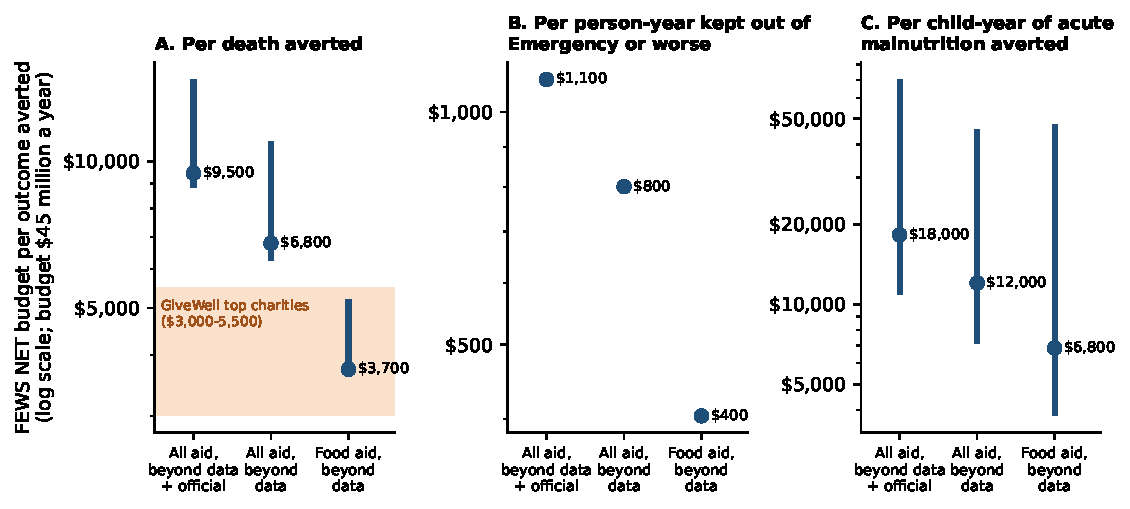
\includegraphics[width=\textwidth]{figures/fig7_benefit_cost.pdf}
\caption{What FEWS NET's budget buys, crediting it only with its distinctive information. Cost per outcome averted, at \$\bcBudget{} million a year, for the aid that follows FEWS NET's forecasts beyond what each country's usual situation, the season, rainfall, conflict and prices predict (``beyond data''), or these plus the latest official analysis (``beyond data + official''), using all humanitarian funding or food and nutrition funding. Dots: central calibration of deaths and malnutrition per phase (Section~\ref{sec:phase}). Bars: range across the low, central and high calibrations. Shaded band: GiveWell's estimate of the cost per death averted by its top charities \citep{givewell2024}.}\label{fig:bcr}
\end{figure}

The calculation leaves out a good deal in both directions.
\begin{itemize}
  \item \textbf{Ways it may overstate.}
    \begin{itemize}
      \item It takes FEWS NET's flags at face value, and nearly half of the flags on failed warnings predate the warning.
      \item Aid that FEWS NET steers may come from other crises where it would also have saved lives. If the displaced aid would have done half as much good, the costs double.
      \item The funding responses are associations, not causal effects.
    \end{itemize}
  \item \textbf{Ways it may understate.}
    \begin{itemize}
      \item FEWS NET's forecasts assume planned aid, which biases its distinctive information downward exactly where aid is flowing.
      \item The calibration of deaths per phase leans on Somalia's scheduled surveys, which under-represent the worst-hit areas, and on phase measures noisy enough to bias the slopes toward zero.
      \item It counts only flagged areas. Crises that warnings prevent entirely never show up, nor do responses by governments, markets and households.
      \item It ignores FEWS NET's value beyond aid allocation, for example to governments, researchers and the official classifications to which its analysts contribute.
    \end{itemize}
\end{itemize}
With those caveats, the calculation puts FEWS NET's distinctive information well below the most cost-effective global health charities in lives saved: \$\bcDistinctLo{}--\bcDistinctHi{} per death averted, against \$3,000--5,500. Measured in food insecurity rather than lives, it does better, at about \$\dCostEmergLo{}--\dCostEmergHi{} per person-year kept out of Emergency. The gap between the two is the central lesson of Section~\ref{sec:phase}: a phase of food insecurity is worth far fewer deaths than the IPC bands suggest.

\paragraph{In a philanthropic funder's units.} Coefficient Giving, a philanthropic funder, compares grants across causes on a common scale \citep{cg2021framework}. The unit is the value of giving \$1 to someone earning \$50,000 a year, and welfare is assumed to rise with the logarithm of income. Raising one person's income by 1 percent for a year is therefore worth about \$500, and a year of healthy life (a disability-adjusted life year, or DALY) is worth \$100,000. A grant clears the funder's bar if it returns roughly 1,000 times its cost in these units, which for health means averting about one DALY per \$100 spent. Averting a death counts as the DALYs it saves. Famine deaths fall heavily on young children, so we assume 30--55 DALYs per death, with 40 as the central case. On that basis FEWS NET's distinctive information returns \cgFortyLo{}--\cgFortyHi{} times its cost across the specifications and mortality scenarios in Table~\ref{tab:bcr}. The range is \cgThirtyLo{}--\cgThirtyHi{} times at 30 DALYs per death and \cgFiftyLo{}--\cgFiftyHi{} times at 55, and \cgBudgetLo{}--\cgBudgetHi{} times across the budget range at the central assumptions. Hunger short of death adds little. Valuing each person-year kept out of Emergency as a 10--25 percent gain in consumption adds \cgHungerLo{}--\cgHungerHi{} times. The bar corresponds to about \$\cgBarPerDeath{} per death averted. On these numbers FEWS NET's distinctive information sits an order of magnitude below the bar. With the IPC bands instead, it would return \ipcCgLo{}--\ipcCgHi{} times its cost, around the bar. Crediting FEWS NET with its whole forecast would give \cgWholeLo{}--\cgWholeHi{} times, which illustrates how much the answer rests on the counterfactual.

\FloatBarrier
\section{Which parts of FEWS NET are worth paying for?}\label{sec:pieces}

The choice facing funders is not only whether to pay for FEWS NET as a whole. FEWS NET bundles several things: field analysts who produce maps and written reports, market price monitoring, and the use of nutrition and mortality surveys run by other agencies. A funder could keep some pieces and not others, or pay to strengthen one. This section asks which of them carry information that improves forecasts. We use two exercises: a pilot that turns FEWS NET's written reports into data, and a test of how much market prices add.

\subsection{The written reports}

FEWS NET publishes far more than maps. Each outlook sets out the assumptions behind the forecast, a worst case, the aid expected and the data the analysts relied on, and updates, key messages and alerts follow between rounds. If the maps compress this reasoning too far, the text might hold early signs of the step FEWS NET forecasts worst, from Crisis to Emergency (Section~\ref{sec:type2}).

We tested this for Somalia, Ethiopia and Sudan, 2011--2024. We downloaded all \txtReports{} of FEWS NET's reports for these countries, including \txtOutlooks{} full outlooks, and used a large language model (Claude) to turn each into structured records. For each area discussed, we recorded the phases stated now and for the projection, any worst case, the expected direction, the drivers named, the status of aid and any statement that data were missing. We also recorded every survey result the report quotes. The model was told to record only what each report says. This matters because the model knows how these crises turned out. Recording stated facts is safe, but asking the model to forecast past crises would not be. Each area is matched to FEWS NET's mapping units by name. As a check, where a report names a district or livelihood zone, the current phase it states lies within the phases on FEWS NET's map for those units in \txtMatch{} percent of \txtMatchN{} cases.

The text adds little to the maps. Of \txtEscN{} area-rounds in Crisis, \txtEscEvents{} reached Emergency on the next map; FEWS NET had forecast Emergency for \txtEscFcFour{} percent of them. We add everything extracted from the reports to FEWS NET's forecast and aid flags: projected Emergency, worst cases, expected deterioration, expected cuts in aid, access constraints, the drivers named and statements of uncertainty. The cross-fitted AUC for escalation does not rise (\txtAucMap{} with the map alone, \txtAucMapText{} with the text). Scored by need, it barely moves (\txtAucNeed{} to \txtAucNeedText{}). Within country and round, two features of the text are associated with escalation (Appendix Table~\ref{tab:text}). Areas where a report expected aid to fall, or said access was constrained, were \txtAidDown{} and \txtAccess{} percentage points more likely to reach Emergency, against a base of \nsEscBase{} percent. Both concern the assumption that planned aid will arrive, which FEWS NET's forecasts build in. But neither improves out-of-sample prediction by more than a hundredth of AUC. The same analysts write the reports and draw the maps, and the two mostly say the same thing. What FEWS NET knows is largely already in its maps. Mining its reports is not a route to much better forecasts, though where its reports doubt the aid pipeline, its forecasts deserve less confidence.

\subsection{Surveys}

The reports do contain something the maps do not: the results of nutrition and mortality surveys. These are mostly standardized SMART surveys run by UNICEF, NGOs and national partners, and in Somalia by the FAO-managed Food Security and Nutrition Analysis Unit. We extracted \svTotal{} distinct survey results (\svSO{} in Somalia, \svET{} in Ethiopia and \svSD{} in Sudan). They measure outcomes independently of any phase classification. Mean acute malnutrition among children under five rises with FEWS NET's phase at the time of the survey: \svGamTwo{} percent in Stressed areas, \svGamThree{} percent in Crisis, \svGamFour{} percent in Emergency and \svGamFive{} percent in Famine. The reports quote surveys selectively, and \svCritShare{} percent of those quoted show acute malnutrition of 15 percent or more. So these results cannot score FEWS NET's accuracy, but they show its phases track measured malnutrition.

Survey coverage is uneven. Among area-rounds that FEWS NET mapped as Emergency, the reports quote a survey from the previous 12 months for \svEmergET{} percent in Ethiopia, \svEmergSO{} percent in Somalia and \svEmergSD{} percent in Sudan. These are lower bounds, since the reports do not quote every survey.

New surveys move the maps, and only upward. In \nsShare{} percent of area-rounds, a survey was carried out between FEWS NET's forecast and its next map. When one was, the next map was worse than the forecast \nsUp{} percentage points more often (standard error \nsUpSe{}, against a base rate of \nsUpBase{} percent). This comparison is within country and round, holds the forecast fixed, and controls for everything the reports said about the area when the forecast was made. The next map was no more likely to be better than forecast (\nsDown{} points, standard error \nsDownSe{}). Among areas in Crisis, a new survey raised the chance of moving to Emergency by \nsEsc{} points (standard error \nsEscSe{}) from a base of \nsEscBase{} percent. A survey preceded \nsUnforecast{} percent of the escalations FEWS NET had not forecast, \nsForecast{} percent of those it had, and \nsNone{} percent of the cases in Crisis that did not escalate.

Three readings could explain this. Surveys may reveal deterioration that the forecast missed. The IPC's rules may cap classifications without survey evidence, so that a survey can unlock a higher phase but its absence rarely pulls one down. Or surveys may be sent where people on the ground already suspect trouble, for reasons the reports do not state. Two checks favor the third reading. First, the rules do not explain it. The IPC requires nutrition and mortality evidence to classify Famine, and weighs it heavily for Emergency, but not for Crisis. Yet among areas forecast to be Stressed or better, a new survey raised the chance that the next map showed Crisis or worse by \nsStressUp{} percentage points (standard error \nsStressUpSe{}, base rate \nsStressBase{} percent). Second, what the survey found matters little. Surveys showing acute malnutrition below 15 percent (\nsOkN{} area-rounds) raised the chance of a worse map by \nsOkUp{} points (standard error \nsOkUpSe{}), about as much as surveys showing 15 percent or more (\nsCritUp{}, standard error \nsCritUpSe{}). If surveys moved the maps through their content, reassuring results would pull them down. Instead they made a better-than-forecast map less likely, not more (\nsOkDown{} points, standard error \nsOkDownSe{}).

So the decision to survey is itself the signal. Agencies send survey teams where conditions are slipping, and FEWS NET's next map moves with them. This tells us two things. First, the people who commission surveys know something FEWS NET's forecasts do not yet reflect. A record of where surveys are planned and why could serve as an early warning in its own right. Second, comparing places with and without surveys cannot show what better survey coverage would add to forecasts, because surveys are not placed at random. That question needs surveys whose timing is fixed in advance, such as scheduled seasonal assessments, so that their results, not the decision to collect them, can be scored. Section~\ref{sec:phase} uses Somalia's scheduled surveys to do this.

\subsection{Market prices}

FEWS NET's data warehouse publishes retail prices from \prMarketsFews{} markets that it monitors itself or compiles from government systems, beyond those it takes from WFP; \prShareNonWfp{} percent of its staple price records are not from WFP. For each area and round, we take 3- and 12-month changes in staple prices at the nearest reporting market within 150 kilometers. WFP and FEWS NET both have a price series for \prBoth{} percent of area-rounds, only WFP for \prWfpOnly{} percent, only FEWS NET for \prFewsOnly{} percent, and neither for \prNone{} percent. FEWS NET's own monitoring fills WFP's gaps in Kenya, Guatemala, parts of Sudan, and Ethiopia in 2016--2019. WFP's data are better in the Sahel, where FEWS NET's prices are not public.

Prices add little to forecasts from either source. We predict which areas tip into Crisis, or escalate from Crisis to Emergency, at the next map, with cross-fitted models. Using only what a donor could see without FEWS NET --- the country, the season, rainfall and political violence --- the AUC for new crises is \pvNewRaw{}; adding both price series gives \pvNewRawBoth{}, while adding FEWS NET's map and forecast gives \pvNewRawMap{}. For escalation the figures are \pvEscRaw{}, \pvEscRawBoth{} and \pvEscRawMap{}. Starting instead from FEWS NET's current and previous maps, prices move the AUC for new crises from \pvNewBase{} to \pvNewBoth{} and for escalation from \pvEscBase{} to between \pvEscBoth{} and \pvEscWfp{}, against \pvNewFc{} and \pvEscFc{} with FEWS NET's forecast. Price changes, taken on their own, carry little of the signal FEWS NET adds. That does not mean prices are worthless: FEWS NET's analysts use them, along with trade flows, terms of trade and household purchasing power, and we cannot test what their judgment would be without them.

Figure~\ref{fig:information} brings the forecasting results together. Panel A shows how much each source of information raises the AUC, starting either from what a donor could see without FEWS NET or from FEWS NET's current maps. Prices and report text add nothing distinguishable from zero. FEWS NET's own map and forecast add \infoMapNew{} points over public data for new crises and \infoMapEsc{} for escalation, and its forecast adds \infoFcNew{} and \infoFcEsc{} points over its current maps. Panel B shows the one input that does move FEWS NET's maps: new survey results.

\begin{figure}[t]
\centering
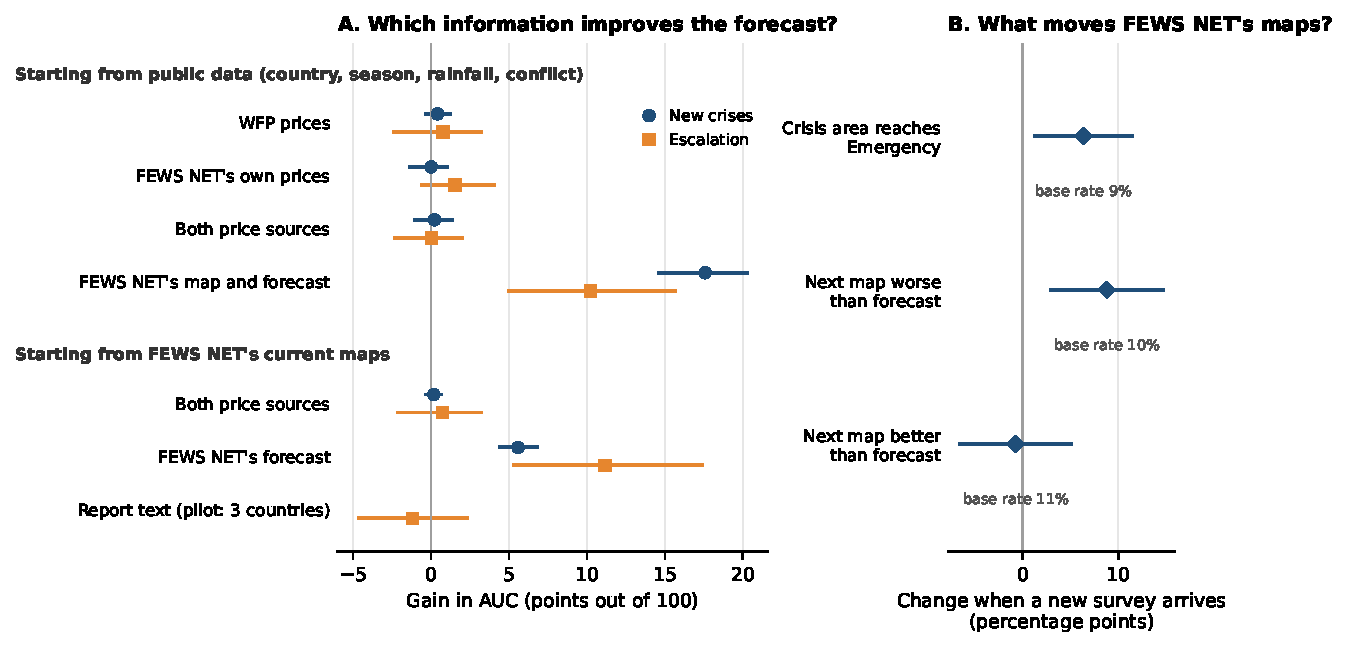
\includegraphics[width=\textwidth]{figures/fig8_information.pdf}
\caption{Which information improves forecasts of food crises? Panel A: gain in the cross-fitted AUC from adding each source of information, for areas tipping into Crisis or worse at the next FEWS NET map (circles) and for areas in Crisis escalating to Emergency or worse (squares), FEWS NET areas 2011--2024. Public data: country, calendar month, forecast horizon, rainfall (CHIRPS) and political violence (ACLED). Prices: 3- and 12-month changes in retail staple prices at the nearest market within 150 km, from WFP or from FEWS NET's own price monitoring and the government systems it compiles. Report text: features extracted from FEWS NET's written reports, Somalia, Ethiopia and Sudan only. Lines are 95 percent intervals from resampling country-years. Panel B: change in the probability of each outcome on the next map when a nutrition or mortality survey is carried out between FEWS NET's forecast and that map, Somalia, Ethiopia and Sudan, with country-by-round fixed effects and controls for the forecast and for everything the reports said about the area at the time; 95 percent intervals clustered by region.}\label{fig:information}
\end{figure}

\subsection{What this means for funding}

The evidence points to three conclusions about the pieces. First, the value lies in the analysts' judgment, not in any data series a funder could buy separately. The part of FEWS NET's forecasts that public data cannot reproduce is the part that is borne out by independent assessments (Section~\ref{sec:value}) and the part that money follows (Section~\ref{sec:money}). Neither prices nor the written reports add much to it. Second, price monitoring is partly duplicative: WFP covers most of the same ground, and together the two leave about one area-round in nine without a nearby price series. FEWS NET's own price monitoring matters most where WFP's is thin. Third, the input most clearly missing is outcome measurement in crisis areas. New surveys are what most often change FEWS NET's classifications, and they are scarcest where crises are hardest to reach. Where surveys are fielded on a schedule, as in Somalia, last season's results predict where children will be malnourished next season far better than FEWS NET's forecasts do; FEWS NET's phases carry little information about malnutrition or child mortality. Without such surveys there is also no way to check, afterward, how bad a crisis was. Sudan, where famine was confirmed in 2024, is the clearest case. Household data collection by humanitarian agencies has also been cut since 2025 \citep{kenny2026drought}. This is where the case for independent, repeated surveys in areas at Crisis or worse \citep{kenny2026humanitarian} meets the case for early warning. The same data would make responses possible to evaluate, and, if collected on a schedule, would add the nutrition and mortality signal that phase classifications lack.

\section{Would paying for surveys pay off?}\label{sec:surveys}

If FEWS NET as a whole looks below the bar in lives saved, would more surveys look better? Surveys of acute malnutrition and mortality cost about \$15,000--21,000 for each area estimated in sub-Saharan Africa, and up to \$30,000 in harder settings \citep{unicef_aah2016smart,daher2018smart}. Somalia's scheduled programme surveys about \svvZones{} rural zones a season, plus towns and displaced settlements. For surveys to save lives, a chain of links must hold:
\begin{enumerate}
  \item more surveys give better information about where children are malnourished and dying;
  \item that information makes warnings better, earlier, or simply louder;
  \item better warnings move more aid, or move it to better places;
  \item that aid reduces malnutrition and death.
\end{enumerate}
The evidence on each link is uneven.

\paragraph{1. Information.} Strong. In Somalia, last season's survey predicts this season's acute malnutrition far better than FEWS NET's forecast (Section~\ref{sec:phase}). No other source we examined substitutes for it, and models that try to predict malnutrition without surveys have performed poorly \citep{checchi2022malnut}.

\paragraph{2. Warnings.} Weak, through FEWS NET. FEWS NET's forecasts barely respond to survey results: a zone whose last survey showed 10 more points of acute malnutrition is forecast \fsFcOnLag{} of a phase worse (standard error \fsFcOnLagSe{}). Ad hoc surveys move FEWS NET's maps upward whatever they find (Section~\ref{sec:pieces}), which looks more like added alarm than added accuracy. FEWS NET's phases are about food insecurity, and survey results about malnutrition do not translate into them.

\paragraph{3. Aid.} Mostly outside FEWS NET. Money follows FEWS NET's forecasts (Section~\ref{sec:money}), but surveys hardly shape those forecasts. Survey results reach aid more directly: nutrition programmes size their caseloads and supplies from survey prevalence, multiplying the number of children by the measured rate and a correction for new cases \citep{isanaka2021icf,bongassie2021afg}. How far donors follow such assessments is less clear \citep{olin2014sida}.

\paragraph{4. Lives.} Strong, for treatment. Treating severe acute malnutrition in the community is among the best-evidenced interventions in crises, at roughly \$4,000--7,000 per death averted when we apply GiveWell's inputs for two well-run programmes \citep{givewell2024cmam,givewell2024taimaka}. But programmes reach a minority of cases; average coverage across 21 countries was 38 percent \citep{rogers2015coverage}.

\paragraph{A targeting calculation.} The most direct route from surveys to lives is helping treatment reach the places with the most malnourished children. We test it in Somalia. Each season, suppose a programme can serve half of the surveyed rural zones and chooses those with the most predicted cases, using either last season's survey or FEWS NET's forecast. Counting the malnourished children actually present in the chosen zones, the survey-based choice covers \svvSurvey{} percent of the season's caseload and the forecast-based choice \svvFc{} percent, against \svvRand{} percent for a random half and \svvOracle{} percent with perfect foresight. Surveys add almost nothing, because where malnourished children are depends mostly on where children are: population size, which both choices use, swamps the differences in rates. At a cost of about \$\svvRound{} a round, the extra children reached would avert about \svvDeaths{} deaths a season, or roughly \$\svvCostMid{} per death (\$\svvCostLo{}--\svvCostHi{} across assumptions on coverage, treatment effects and survey costs). If instead programmes are placed by malnutrition rate alone, as prioritization by emergency thresholds does, surveys matter much more: the survey-based choice covers \svvRateSurvey{} percent of the caseload against \svvRateFc{} percent for the forecast, at roughly \$\svvRateMid{} per death (\$\svvRateLo{}--\svvRateHi{}). But a rule that ignores population is a poor one, and its gains come largely from correcting that.

\paragraph{What this implies.} The case for paying for more surveys does not rest on better FEWS NET warnings, and in Somalia it does not rest on better geographic targeting either: knowing population size gets most of the way. It rests on three other things that this paper cannot price. First, surveys are the only way to see malnutrition and mortality directly, including famine-level conditions that phases of food insecurity do not reliably signal. Second, they size the response: how much therapeutic food to buy and how many staff to deploy depend on measured rates, not phases. Third, they are the only way to know afterwards whether a response worked, which is what the debate over aid cuts lacks \citep{kenny2026humanitarian}. A test of the second would need data on procurement and stock-outs; a test of the third, a funder willing to treat surveys as evaluation infrastructure rather than as early warning.

\FloatBarrier
\FloatBarrier
\section{What the data cannot tell us}\label{sec:limits}\label{sec:limits2}

The ideal evaluation would compare welfare --- child malnutrition, mortality --- in places and times with and without FEWS NET. We tried two versions with the data available, and neither is informative.

\paragraph{The 2025 shutdown.} FEWS NET went dark in January 2025 just as U.S. aid was cut. If its ``held back by aid'' flags are right, flagged areas should have deteriorated faster afterwards than comparable unflagged areas. Over 12 months, flagged areas worsen relative to comparable unflagged areas by about \flagOwnPlacebo{} of a phase in normal years. For windows ending in 2025, the gap widened by a further \flagOwn{} phases on FEWS NET's own later maps (wild bootstrap $p = \flagOwnP{}$) and \flagIpc{} on official classifications ($p = \flagIpcP{}$). The flag carries information about fragility, but the data cannot yet separate the cut's effect from the trend. We need outcomes beyond mid-2026 (Appendix~\ref{app:shutdown}).

\paragraph{Changes in FEWS NET coverage.} FEWS NET has entered and left countries over time, but these moves follow aid and conflict trends, so comparing levels before and after is confounded. A narrower test asks whether local shocks do less damage, within a country, when FEWS NET covers it. Local rainfall, conflict and price shocks explain only \shockRsq{} percent of the variation in official classifications within country and month, and coverage does not change their effect (\covPre{}, standard error \covPreSe{}, before 2025). Classifications move too slowly, and too nationally, to detect FEWS NET's effect this way (Appendix~\ref{app:coverage}). The same weakness of public fundamentals appears in Section~\ref{sec:money}: they explain little of FEWS NET's forecasts within a country and season, which is why most of FEWS NET's information cannot be reproduced from public data.

Testing whether FEWS NET saves lives will require outcomes it does not produce: child anthropometry and mortality from household surveys, linked to the timing and location of its warnings.

\section{Conclusion}\label{sec:conclusion}

FEWS NET rarely misses a food crisis outright, but it often sees emergencies late and one phase too mild. About half of its emergency warnings do not come true; FEWS NET credits aid for about half of those, though often aid that was already flowing. Measured against what donors could otherwise know, it adds information that independent assessments later bear out, it raises fewer false alarms than the official projections, and humanitarian funding moves with the part of its forecasts that public data cannot reproduce.

For funders deciding FEWS NET's future, the relevant comparison is with what would replace it. In three-quarters of FEWS NET's coverage, there is no recent official analysis to fall back on, and the raw signals --- rainfall, conflict, prices --- predict where crises will strike much less well. FEWS NET's distinctive contribution is modest in any single forecast but systematic, and it is the part that money follows. Against a budget of about \$\bcBudget{} million a year --- a fraction of a percent of the humanitarian funding that flows to the countries it monitors --- a rough calculation that credits FEWS NET only with its distinctive information, and takes its own judgments of what aid prevents at face value, puts its cost at \$\bcDistinctLo{}--\bcDistinctHi{} per death averted and \$\dCostEmergLo{}--\dCostEmergHi{} per person-year kept out of Emergency. As a way of saving lives, that is well below the best alternatives. The reason is less FEWS NET's skill than what it measures: a phase of food insecurity is worth far fewer deaths than the IPC's reference bands imply, and evaluations that use the bands, as this one first did, overstate the lives at stake by several times.

For funders choosing among pieces rather than the whole, the value lies in the analysts' judgment. Neither FEWS NET's written reports nor market price series add much to what its maps already say. The piece most clearly missing is outcome measurement: new nutrition and mortality surveys are what most often change FEWS NET's maps, and they are scarcest in places like Sudan, where they matter most. Paying for repeated surveys in areas at Crisis or worse would make it possible to tell, afterward, whether the response worked. In Somalia, where surveys already run on a fixed schedule, last season's results predict this season's child malnutrition far better than FEWS NET's forecasts, which barely track it at all. Warnings about food insecurity and warnings about malnutrition and death are different products, and only surveys supply the second. But surveys do not obviously pay for themselves through better targeting: in Somalia, knowing where children live gets treatment most of the way to where malnourished children are. Their value lies in sizing responses, in seeing famine-level conditions directly, and in making it possible to know whether a response worked.

Three changes would make the system easier to evaluate and probably more useful. First, publish a forecast without assumed aid alongside the current one. Donors need to know what will happen if they do nothing, and evaluators need it to separate crises prevented from false alarms. Second, record when and why the aid flag is applied, so that ``held back by aid'' can be distinguished from ``aid was already there.'' Third, validate forecasts against independent outcomes. Our comparisons use the IPC and Cadre Harmonis\'e, which share analysts with FEWS NET; linking FEWS NET's warnings to household survey data on child malnutrition and mortality would show whether its information, and the aid it moves, change lives.

\newpage
\bibliographystyle{chicago}
\bibliography{references}

\newpage
\begin{appendices}
\renewcommand{\thefigure}{A\arabic{figure}}
\renewcommand{\thetable}{A\arabic{table}}
\setcounter{figure}{0}
\setcounter{table}{0}

\section{Data construction}\label{app:data}

\paragraph{FEWS NET classifications.} We download all current-situation (``CS'') and projection (``ML1'' near-term, ``ML2'' medium-term) classifications from the FEWS NET Data Warehouse, month by month, January 2011 to August 2026, and use those through December 2024. Each record gives an area identifier, its phase, the projection period and whether the area carries the aid flag. We use the full map rounds (three per year since 2016; quarterly before). For the analyses in Sections~\ref{sec:value} and~\ref{sec:money}, the unit is an area and map round, giving \panelAreaRounds{} area-rounds for \panelAreas{} areas in \panelCountries{} countries with complete forecasts and a next map within eight months.

\paragraph{Official classifications.} Cadre Harmonis\'e records (current and projected) come from the regional dataset; IPC records from the IPC's area-level data (2017--2026). For IPC records we derive the area phase from population shares using the IPC's 20 percent rule. Areas are matched to polygons from the Cadre Harmonis\'e 2023 map, IPC country maps and geoBoundaries administrative units, and overlaid on FEWS NET's areas in an equal-area projection. FEWS NET's classifications are averaged over each official area, weighted by overlap.

\paragraph{Raw signals.} Rainfall is the area mean of monthly CHIRPS rainfall. Conflict is ACLED's district-level political violence data, available sub-nationally for the 19 countries with UN humanitarian response plans. Districts are matched to OCHA administrative boundaries by district code, then by name, and apportioned to FEWS NET areas by area share. Prices are the mean 3- and 12-month log changes of retail cereal and tuber prices at the WFP market nearest each FEWS NET area, within 150 km.

\paragraph{Funding.} Humanitarian commitments (``paid'' and ``commitment'' status, incoming flows) from the Financial Tracking Service, assigned to recipient countries; multi-country flows are dropped. Food and nutrition funding is the subset whose cluster is Food Security or Nutrition.

\paragraph{Prediction models.} All benchmark predictions use gradient-boosted trees (scikit-learn's histogram gradient boosting) with country as a categorical feature, cross-fitted by year: predictions for each year come from a model trained on all other years.

\section{The masking test}\label{app:masking}

If aid prevents crises that FEWS NET warns about, its distinctive warnings should be borne out less often when funding to the country rises unexpectedly. Funding surprises are country-round residuals of log funding over the next six months, after removing country and time effects and the country's funding in the previous six months. We split country-rounds into thirds and estimate, within each third, how much of FEWS NET's distinctive warning (the forecast minus its prediction from raw signals and previous maps) is borne out on its next map, with country-by-round fixed effects. Figure~\ref{fig:masking} shows no pattern: the share is about one half in all three groups, whether outcomes are scored as mapped or by need. The interaction of the distinctive warning with the funding surprise is \maskInter{} (standard error \maskInterSe{}).

\begin{figure}[H]
\centering
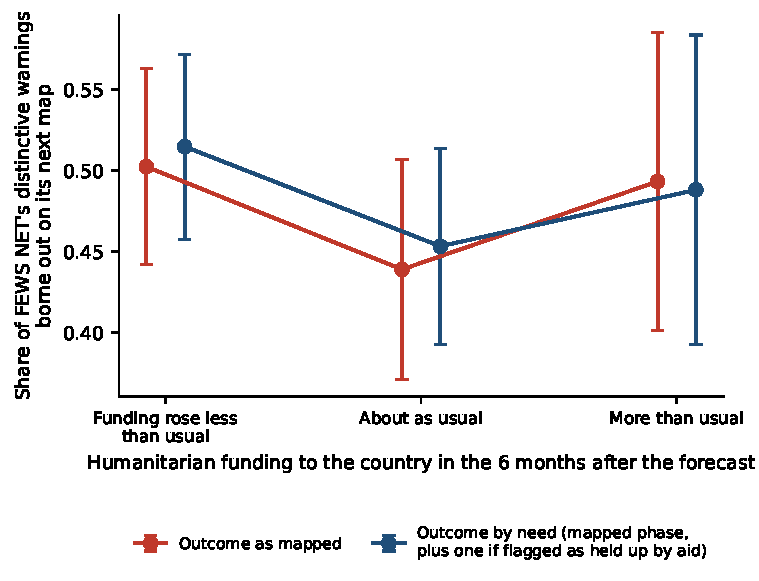
\includegraphics[width=0.7\textwidth]{figures/figA1_masking.pdf}
\caption{Do warnings come true less often where money flowed? Coefficient on FEWS NET's distinctive warning (forecast of Crisis or worse minus its out-of-sample prediction from rainfall, conflict, prices, previous maps, country and season) in a regression of Crisis or worse on its next map, by the country's funding surprise over the following six months. Red: outcome as mapped. Blue: outcome by need (mapped phase plus one if flagged as held up by aid). 95 percent intervals clustered by country.}\label{fig:masking}
\end{figure}

\section{The 2025 shutdown}\label{app:shutdown}

We compare same-season changes in areas FEWS NET flagged as held up by aid with unflagged areas that started in the same phase, country and month, for 12-month windows ending each year from 2014 to 2025. Windows ending in 2025 span the shutdown and the U.S. aid cut; earlier windows show how flagged areas normally evolve. Figure~\ref{fig:shutdown} shows that flagged areas worsen relative to unflagged ones in almost every year, and that the gap was already rising in 2023--2024, when humanitarian funding was falling. The 2025 gap is in line with that trend. Using 24-month windows produces a larger 2025 gap that is not repeated in 2026; pooling horizons, as in an earlier version of this analysis, mixes windows of different lengths in different years and overstates the effect.

\begin{figure}[H]
\centering
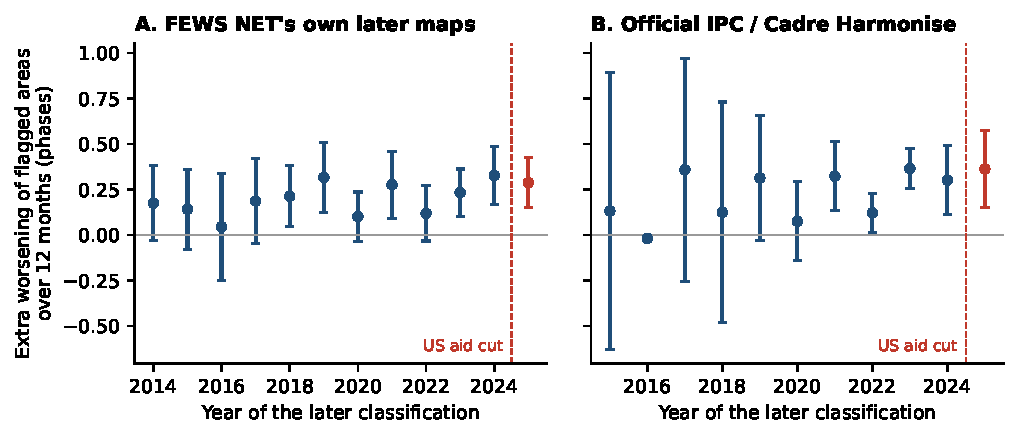
\includegraphics[width=0.85\textwidth]{figures/figA2_shutdown.pdf}
\caption{Did areas FEWS NET flagged as held up by aid deteriorate after the 2025 shutdown? Difference in the 12-month change in phase between flagged and unflagged areas that started in the same phase, country and month, by the year the window ends. Panel A: FEWS NET's own maps (FEWS NET areas in Phase 2--3). Panel B: official IPC and Cadre Harmonis\'e analyses, with the flag measured as the share of the official area covered by flagged FEWS NET areas in a map made at most four months before. Red: windows ending after the shutdown. 95 percent intervals clustered by country.}\label{fig:shutdown}
\end{figure}

\section{Coverage changes and local shocks}\label{app:coverage}

We built an index of local shocks --- rainfall deficits, political violence and food price spikes, weighted to predict official classifications in other countries --- and asked whether its effect on official classifications differs, within a country, between periods when FEWS NET covered the country and periods when it did not. With area and country-by-month fixed effects and country-specific shock effects, the interaction is \covPre{} (standard error \covPreSe{}) before 2025 and \covPost{} (\covPostSe{}) in 2025--2026, measured on the share of the population in Crisis or worse. The index explains only \shockRsq{} percent of the within-country variation in classifications; rainfall alone explains \shockRsqRain{} percent. An earlier specification suggested that shocks did \emph{more} damage under FEWS NET coverage; that result rested entirely on Cameroon, where FEWS NET arrived in 2020 as conflict escalated, and on archive gaps that made FEWS NET appear to leave Burkina Faso and Mauritania when it had not.

\section{Funding regressions}\label{app:money}

\begin{table}[H]
\centering

\caption{Humanitarian funding and FEWS NET's maps and forecasts, within countries}\label{tab:money}
\scriptsize
\resizebox{\textwidth}{!}{\begin{tabular}{lcccccc}
\toprule
 & \multicolumn{2}{c}{Map vs forecast} & \multicolumn{2}{c}{Beyond rainfall,} & \multicolumn{2}{c}{Beyond rainfall, conflict,} \\
 & \multicolumn{2}{c}{} & \multicolumn{2}{c}{conflict and prices} & \multicolumn{2}{c}{prices and official analysis} \\
\cmidrule(lr){2-3}\cmidrule(lr){4-5}\cmidrule(lr){6-7}
 & All & Food & All & Food & All & Food \\
 & (1) & (2) & (3) & (4) & (5) & (6) \\
\midrule
Share of areas in Crisis+, current map & $-1.0$ & $-1.8$ &  &  &  &  \\
 & $(4.0)$ & $(6.7)$ &  &  &  &  \\
Share of areas forecast in Crisis+ & $10.0^{***}$ & $22.1^{**}$ &  &  &  &  \\
 & $(3.8)$ & $(8.6)$ &  &  &  &  \\
Forecast: part predictable from country, season and shocks &  &  & $3.1$ & $9.7$ & $6.7$ & $16.3$ \\
 &  &  & $(6.7)$ & $(14.5)$ & $(6.2)$ & $(12.8)$ \\
Forecast: FEWS NET's own contribution &  &  & $11.2^{***}$ & $28.3^{***}$ & $10.2^{***}$ & $26.9^{***}$ \\
 &  &  & $(3.9)$ & $(9.3)$ & $(3.6)$ & $(9.4)$ \\
\midrule
Country $\times$ map rounds & 968 & 967 & 851 & 850 & 851 & 850 \\
Countries & 37 & 37 & 28 & 28 & 28 & 28 \\
\bottomrule
\end{tabular}}
\par\vspace{4pt}\begin{minipage}{\textwidth}\scriptsize \textit{Notes:} Country $\times$ FEWS NET map round, 2011--2024. Outcome: log humanitarian funding committed to the country over the six months after the map (OCHA Financial Tracking Service); all humanitarian funding (``All'') or food security and nutrition (``Food''). Coefficients are scaled to log points per 10 percentage points of the country's FEWS NET areas (approximately the percent change). Columns 1--2: share of areas in Crisis or worse on the current map and in the medium-term forecast, in the same regression. Columns 3--6: the forecast share split into its out-of-sample prediction from rainfall, conflict, prices, country and season (columns 3--4), or these plus the latest official analysis (columns 5--6), and FEWS NET's contribution beyond that prediction. All columns include country and time fixed effects and log funding in the previous six months. Standard errors clustered by country in parentheses. * $p<0.10$, ** $p<0.05$, *** $p<0.01$.
\end{minipage}

\end{table}

\section{FEWS NET's reports and escalation}\label{app:text}

\begin{table}[H]
\centering
\caption{Do FEWS NET's reports predict escalation from Crisis to Emergency beyond its maps?}\label{tab:text}
\scriptsize
\resizebox{\textwidth}{!}{\begin{tabular}{lcccccc}
\toprule
 & \multicolumn{3}{c}{Emergency+ on next map} & \multicolumn{3}{c}{Emergency+ by need} \\
\cmidrule(lr){2-4}\cmidrule(lr){5-7}
 & (1) & (2) & (3) & (4) & (5) & (6) \\
\midrule
FEWS NET forecast: Emergency & 0.245*** & 0.242*** & 0.245*** & 0.408*** & 0.409*** & 0.406*** \\
 & (0.040) & (0.037) & (0.036) & (0.062) & (0.062) & (0.060) \\
Aid flag now & 0.033 & 0.033 & 0.035 & 0.253*** & 0.250*** & 0.242*** \\
 & (0.033) & (0.036) & (0.036) & (0.036) & (0.037) & (0.036) \\
Aid flag in forecast & 0.117*** & 0.113*** & 0.114*** & 0.211*** & 0.207*** & 0.197*** \\
 & (0.019) & (0.018) & (0.019) & (0.044) & (0.046) & (0.047) \\
Report: Emergency projected &  & 0.002 & -0.001 &  & 0.003 & -0.001 \\
 &  & (0.030) & (0.031) &  & (0.033) & (0.031) \\
Report: worst case Emergency or Famine &  & 0.000 & -0.001 &  & -0.002 & -0.007 \\
 &  & (0.021) & (0.020) &  & (0.029) & (0.030) \\
Report: deterioration expected &  & -0.025 & -0.026 &  & -0.039 & -0.035 \\
 &  & (0.019) & (0.019) &  & (0.031) & (0.032) \\
Report: aid expected to fall &  & 0.060** & 0.050* &  & 0.063** & 0.050* \\
 &  & (0.030) & (0.027) &  & (0.029) & (0.026) \\
Report: access constrained &  & 0.067*** & 0.059*** &  & 0.037 & 0.031 \\
 &  & (0.024) & (0.022) &  & (0.035) & (0.030) \\
Report: conflict or displacement &  & -0.015 & -0.010 &  & 0.006 & 0.010 \\
 &  & (0.016) & (0.016) &  & (0.019) & (0.021) \\
Report: poor rains or harvest &  & -0.003 & 0.004 &  & -0.005 & 0.005 \\
 &  & (0.034) & (0.031) &  & (0.032) & (0.032) \\
Report: high prices or currency &  & 0.021 & 0.020 &  & 0.003 & 0.004 \\
 &  & (0.020) & (0.020) &  & (0.026) & (0.027) \\
Report: uncertainty stated &  & -0.008 & -0.015 &  & 0.027 & 0.014 \\
 &  & (0.026) & (0.025) &  & (0.050) & (0.053) \\
Area discussed in reports &  & -0.059 & -0.071 &  & -0.081* & -0.098** \\
 &  & (0.050) & (0.049) &  & (0.048) & (0.045) \\
Survey in previous 12 months &  &  & 0.091*** &  &  & 0.127*** \\
 &  &  & (0.029) &  &  & (0.028) \\
Survey: acute malnutrition 15\%+ &  &  & -0.105*** &  &  & -0.044 \\
 &  &  & (0.026) &  &  & (0.035) \\
Survey: death rate above emergency threshold &  &  & 0.072* &  &  & 0.041 \\
 &  &  & (0.040) &  &  & (0.049) \\
Report: data gap stated &  &  & 0.008 &  &  & -0.017 \\
 &  &  & (0.014) &  &  & (0.026) \\
\midrule
Area-rounds & 8,564 & 8,564 & 8,564 & 8,564 & 8,564 & 8,564 \\
\bottomrule
\end{tabular}
}
\par\vspace{4pt}\begin{minipage}{\textwidth}\scriptsize \textit{Notes:} Linear probability models. Sample: FEWS NET areas in Crisis (Phase 3) at map round $r$, Somalia, Ethiopia and Sudan, 2011--2024, in rounds with at least one extracted report. Outcome: Emergency or worse on the next map (columns 1--3), or by need, the mapped phase plus one if flagged as held back by aid (columns 4--6). ``Report'' variables are indicators that a FEWS NET report published in the four months up to $r$ said this about the area (extracted with a large language model and matched to mapping units by name). Survey variables refer to survey results quoted in reports, fielded in the 12 months before $r$. All columns include country-by-round fixed effects. Standard errors clustered by region (first administrative level) in parentheses. * $p<0.10$, ** $p<0.05$, *** $p<0.01$.
\end{minipage}
\end{table}

\section{Replication}\label{app:replication}

All data are public. The analysis is in Python, in the project's \texttt{code} directory.
\begingroup\sloppy\small
\begin{itemize}
  \item FEWS NET data: \texttt{01\_fetch\_fewsnet.py}, \texttt{07\_build\_panel.py}
  \item Official classifications: \texttt{04\_fetch\_ipc\_ch.py}, \texttt{23\_outcome\_panel.py}
  \item Funding: \texttt{03\_fetch\_fts.py}
  \item Rainfall, conflict and prices: \texttt{22\_fetch\_chirps.py}, \texttt{24\_area\_rainfall.py}, \texttt{26\_fetch\_acled\_wfp.py}
  \item Type I and II errors: \texttt{12\_errors.py}; need-defined emergencies: \texttt{30\_need\_onsets.py}
  \item The 2025 shutdown: \texttt{28\_flag\_release.py}; coverage changes: \texttt{27\_shock\_index.py}
  \item Funding responses: \texttt{31\_aid\_response.py}
  \item FEWS NET's distinctive information: \texttt{32\_forecast\_value.py}, \texttt{33\_fewsnet\_contribution.py}
  \item Official projections: \texttt{34\_official\_projections.py}
  \item FEWS NET's reports: \texttt{50\_fetch\_reports.py}, \texttt{51\_extraction\_instructions.md}, \texttt{52\_text\_features.py}, \texttt{53\_text\_value.py}; prices: \texttt{54\_fetch\_fdw\_prices.py}, \texttt{55\_price\_value.py}; Somalia's scheduled surveys: \texttt{56\_fsnau\_surveys.py}, \texttt{57\_fsnau\_value.py}
  \item Numbers, figures and tables in this paper: \texttt{40\_paper.py}, \texttt{41\_paper\_tables.py}, \texttt{42\_paper\_bootstrap.py}
\end{itemize}
\endgroup

\end{appendices}
\end{document}
